%%
%% This is file `sample-sigconf.tex',
%% generated with the docstrip utility.
%%
%% The original source files were:
%%
%% samples.dtx  (with options: `sigconf')
%% 
%% IMPORTANT NOTICE:
%% 
%% For the copyright see the source file.
%% 
%% Any modified versions of this file must be renamed
%% with new filenames distinct from sample-sigconf.tex.
%% 
%% For distribution of the original source see the terms
%% for copying and modification in the file samples.dtx.
%% 
%% This generated file may be distributed as long as the
%% original source files, as listed above, are part of the
%% same distribution. (The sources need not necessarily be
%% in the same archive or directory.)
%%
%% The first command in your LaTeX source must be the \documentclass command.
\documentclass[sigconf]{acmart}

%%
%% \BibTeX command to typeset BibTeX logo in the docs
\AtBeginDocument{%
  \providecommand\BibTeX{{%
    \normalfont B\kern-0.5em{\scshape i\kern-0.25em b}\kern-0.8em\TeX}}}

%% Rights management information.  This information is sent to you
%% when you complete the rights form.  These commands have SAMPLE
%% values in them; it is your responsibility as an author to replace
%% the commands and values with those provided to you when you
%% complete the rights form.
% \setcopyright{acmcopyright}
% \copyrightyear{2018}
% \acmYear{2018}
% \acmDOI{10.1145/1122445.1122456}

%% These commands are for a PROCEEDINGS abstract or paper.
% \acmConference[Woodstock '18]{Woodstock '18: ACM Symposium on Neural
%   Gaze Detection}{June 03--05, 2018}{Woodstock, NY}
% \acmBooktitle{Woodstock '18: ACM Symposium on Neural Gaze Detection,
%   June 03--05, 2018, Woodstock, NY}
% \acmPrice{15.00}
% \acmISBN{978-1-4503-XXXX-X/18/06}


%%
%% Submission ID.
%% Use this when submitting an article to a sponsored event. You'll
%% receive a unique submission ID from the organizers
%% of the event, and this ID should be used as the parameter to this command.
%%\acmSubmissionID{123-A56-BU3}

%%
%% The majority of ACM publications use numbered citations and
%% references.  The command \citestyle{authoryear} switches to the
%% "author year" style.
%%
%% If you are preparing content for an event
%% sponsored by ACM SIGGRAPH, you must use the "author year" style of
%% citations and references.
%% Uncommenting
%% the next command will enable that style.
%%\citestyle{acmauthoryear}

%%
%% end of the preamble, start of the body of the document source.
\begin{document}

%%
%% The "title" command has an optional parameter,
%% allowing the author to define a "short title" to be used in page headers.
\title{Extending and Experimenting with the EvoSuite Test Generation Tool}

%%
%% The "author" command and its associated commands are used to define
%% the authors and their affiliations.
%% Of note is the shared affiliation of the first two authors, and the
%% "authornote" and "authornotemark" commands
%% used to denote shared contribution to the research.
\author{Aidin Rasti}
% \authornote{Both authors contributed equally to this research.}
\email{arast040@uottawa.ca}
% \orcid{1234-5678-9012}
% \author{G.K.M. Tobin}
% \authornotemark[1]
% \email{webmaster@marysville-ohio.com}
\affiliation{%
  \institution{University of Ottawa}
  % \streetaddress{P.O. Box 1212}
  \city{Ottawa}
  \state{Ontario}
  \country{Canada}
  % \postcode{43017-6221}
}

%%
%% By default, the full list of authors will be used in the page
%% headers. Often, this list is too long, and will overlap
%% other information printed in the page headers. This command allows
%% the author to define a more concise list
%% of authors' names for this purpose.
\renewcommand{\shortauthors}{Aidin}

%%
%% The abstract is a short summary of the work to be presented in the
%% article.
\begin{abstract}
  Search-based test generation techniques are one of the effective test generation approaches. 
  EVOSUITE is one of the whole test suite generation tools that has implemented several 
  types of Genetic Algorithms. We compare and show the results of generating tests for ten open-source 
  Java projects with a combination of different selection and crossover functions in EVOSUITE. 
  We have also extended EVOSUITE and implemented the two-point crossover function.
\end{abstract}


%%
%% The code below is generated by the tool at http://dl.acm.org/ccs.cfm.
%% Please copy and paste the code instead of the example below.
%%
\begin{CCSXML}
<ccs2012>
   <concept>
       <concept_id>10011007.10011074.10011784</concept_id>
       <concept_desc>Software and its engineering~Search-based software engineering</concept_desc>
       <concept_significance>500</concept_significance>
       </concept>
   <concept>
       <concept_id>10002944.10011123.10010912</concept_id>
       <concept_desc>General and reference~Empirical studies</concept_desc>
       <concept_significance>500</concept_significance>
       </concept>
   <concept>
       <concept_id>10010147.10010257.10010293.10011809.10011812</concept_id>
       <concept_desc>Computing methodologies~Genetic algorithms</concept_desc>
       <concept_significance>500</concept_significance>
       </concept>
 </ccs2012>
\end{CCSXML}

\ccsdesc[500]{Software and its engineering~Search-based software engineering}
\ccsdesc[500]{General and reference~Empirical studies}
\ccsdesc[500]{Computing methodologies~Genetic algorithms}

%%
%% Keywords. The author(s) should pick words that accurately describe
%% the work being presented. Separate the keywords with commas.
\keywords{genetic algorithms, test generation, search-based software engineering, empirical evaluation}

%% A "teaser" image appears between the author and affiliation
%% information and the body of the document, and typically spans the
%% page.
% \begin{teaserfigure}
%   \includegraphics[width=\textwidth]{sampleteaser}
%   \caption{Seattle Mariners at Spring Training, 2010.}
%   \Description{Enjoying the baseball game from the third-base
%   seats. Ichiro Suzuki preparing to bat.}
%   \label{fig:teaser}
% \end{teaserfigure}

%%
%% This command processes the author and affiliation and title
%% information and builds the first part of the formatted document.
\maketitle

\section{Introduction}
Search-Based Software Engineering (SBSE) has numerous use cases \cite{10.1145/2379776.2379787,Harman2012}.
One of the exciting applications of SBSE is automated unit test generation. There are several works on this
subject \cite{57624,6004309,10.1145/1276958.1277172,10.1145/1013886.1007528}. One of the methods of automated
unit test generation is using Genetic Algorithms. EVOSUITE \cite{6004309} is 
a novel evolutionary-based approach for whole test suit generation. There are two approaches to search 
based test generation, one is targeting a single criterion at a time, for example, targeting each branch
individually and generating data for that particular target branch. The other approach is generating and 
optimizing the whole test suit at the same time while maximizing coverage and minimizing test suite size. 
Instead of generating tests for each target goal one at a time, it generates and optimizes a whole test suite 
simultaneously. 

EVOSUITE is a solution in the latter category, it is a whole test suite generation solution that can
target multiple criteria at the same time. EVOSUITE starts with a random set of initial solutions and uses 
an evolutionary approach to improve solutions until the chosen criteria are satisfied.
After generating solutions it will minimize the test suite size. EVOSUITE is developed in Java. Currently, 
it only generates tests in the JUnit format for Java programs. EVOSUITE works by instrumenting the compiled 
java bytecode and collecting metrics from the runtime. EVOSUITE is designed to write tests 
for object-oriented programs, therefore it can comfortably generate tests for a Class, 
which may require a sequence of method calls. 

Genetic Algorithms are used to optimize and evolve a set of initial solutions toward better fitness values.
Like all search-based techniques, Genetic Algorithms also have a solution representation and fitness function 
defined for the problem at hand. A typical flow of a Genetic Algorithm is as follows. 
The first step is the initialization, one way to do this is to randomly generate initial solutions. After calculating
the fitness of each solution, a few of them are selected to create offsprings. This is called 
the Selection step. One method to do selection is to simply choose solutions with the best fitness values.
After selecting parents, offsprings are created by applying a Crossover function. A popular way of doing crossover
is to simply flip parents at a point and select before/after the point for each child. For example, suppose
our solution is represented as an array of numbers and we have selected the middle of the array as the flipping point.
From the beginning to the middle of the first parent and from the middle to the end of
the second parent goes to the first child, and vice versa for the second child. After breeding a new generation of
solutions mutations operators are applied to solutions. Mutation operators depend on the problem and 
solution representation. This process from fitness evaluation to mutations continues until termination criteria
are met or appropriate solutions are found.

EVOSUITE is a highly configurable software, users can tweak its numerous parameters to achieve the best result. 
Authors of EVOSUITE have implemented several variations of Genetic Algorithms. In this report, we compare 
a variety of different crossover and selection functions for the standard genetic algorithm implemented in EVOSUITE.
We used the standard Genetic Algorithm as the base and evaluated the performance of 
Uniform, Single point, and Two-point crossover functions in combination with Rank, Roulette Wheel, Tournament, 
and Best-k selection methods. Therefore we have eight combination of configurations to evaluate. 
EVOSUITE does not include the Two-point crossover function and we have implemented it.
We have selected ten popular and open-source Java libraries from GitHub for our tests.

The structure of this report is as follows. First, in Section \ref{relatedworks} we introduce other
empirical works related to test generation with EVOSUITE then in Section \ref{experiments} we describe
our testing approach, we explain our test configurations and procedure. Also, we briefly describe each of
our test subjects. Finally, in Section \ref{evaluation} we show the result of our evaluations.

\section{Related Works}
\label{relatedworks}
One of the most comprehensive work that evaluates the performance of EVOSUITE is \cite{CAMPOS2018207}. They have
compared the performance of different test generation algorithms, such as Standard GA, Monotonic GA, 
DynaMOSA \cite{7840029}, MIO \cite{Arcuri_2017}, etc, in EVOSUITE. 
Their tests include both single objective and multi-objective evaluations. They have concluded that
DynaMOSA has the most covered targets in both single and multi-objective scenarios. The goal of their work is
to compare different test generation algorithms, however, we want to compare the performance of different crossover
and selection methods. We have used the Standard GA as our base algorithm and assessed the results under different
configurations.

Another comprehensive work is the work of Arcuri and Fraser \cite{Tuning13} which evaluates several 
hyperparameters of EVOSUITE and the effect of parameter tuning in test generation problems in general.
They are more concerned with the effect of parameters like population size, crossover rate, probability
configurations, search budget, etc. 

Another work is \cite{emse16_effectiveness} which compares the traditional single criterion approaches
with multi-objective approaches available in EVOSUITE. Traditionally test generation solutions take
a single criterion like branch coverage to generate unit tests. In newer whole test suite generation 
approaches several criteria like line coverage, branch coverage, etc can be used by algorithms 
like DynaMOSA \cite{7840029} at the same time. 
These algorithms optimize for all of the targets at the same time. Their work concluded
that there may be a small set of targets that may not be covered by multi-objective approaches.

One more empirical work is \cite{STVR_seeding} that evaluates several seeding strategies for test generation
problems. Seeding is the problem of providing values for method and class parameters when generating or
modifying unit tests in search-based techniques. There are several solutions for seeding. For example, 
one way is to randomly use available constant values in the source code as input parameters.
Another way is to observe passed parameters during runtime and use them during test generation. They have concluded 
that the choice of seeding strategy can impact the performance of search-based test generation solutions.

\section{Experiments}
\label{experiments}
We have used the EVOSUITE test generation tool to compare the performance of several crossover 
and selection functions with the standard Genetic Algorithm. 
In total, our evaluations included 165 Java classes from various popular open-source projects 
and we have performed 12,240 tests. 

\subsection{Configurations}
As mentioned earlier we have a total of eight configurations to compare. We have tested the performance
of EVOSUITE by changing its crossover and selection functions. These two are
denoted respectively by \verb|crossover_function| and \verb|selection_function| in EVOSUITE parameters. 
We have only used the standard GA, which is denoted by the configuration value \verb|STANDARD_GA| in EVOSUITE.
In the followed subsections we briefly describe each algorithm that we have tested.

\subsubsection{Selection methods}
Selection is one of the stages in a genetic algorithm. In this stage, a number of pairs of parents
are selected to build offsprings. There are several selection methods available for use in genetic algorithms.
We assessed four selection methods implemented in EVOSUITE, Rank Selection, Roulette Wheel, Tournament Selection, 
and Best-k.
\begin{itemize}
  \item{Roulette Wheel}: In this method each individual is given a probability of selection equal to 
  their fitness values, therefore, better individuals have a much higher chance of being selected. It is denoted
  by \verb|ROULETTEWHEEL| value in EVOSUITE properties.
  \item{Rank Selection}: In Rank selection, parents are first sorted according to their fitness 
  value and then each is given a probability of selection equal to their rank. Its advantage over 
  Roulette Wheel is that it still gives individuals with a low fitness value a chance of being selected.
  In Roulette Wheel individuals with a high fitness value fill much more proportion of the probability space,
  but Rank Selection fixes this problem. It is denoted by \verb|RANK| value in EVOSUITE properties.
  \item{Tournament Slection}: Individual chromosomes of the population are matched against each other
  in a tournament fashion and the winners are selected for crossover. It is denoted
  by \verb|TOURNAMENT| value in EVOSUITE properties.
  \item{Best-k}: Selects the k top parents based on their fitness values. It is denoted
  by \verb|BESTK| value in EVOSUITE properties.
\end{itemize}

\subsubsection{Crossover methods}
After choosing parents by applying a selection method, offsprings are created from parents by using a
crossover function. There are several crossover functions proposed for use in Genetic Algorithms. We evaluated
the performance of Uniform, Relative Single Point, and Two-point crossover functions implemented in EVOSUITE. We have 
extended EVOSUITE and implemented the two-point crossover method.
\begin{itemize}
  \item{Relative Single Point}: This method is like the standard Single Point crossover function,
  however, in the Relative Single Point, the size of individuals is also taken into account. For example, If we want
  to select half of each parent and perform crossover, then for a chromosome of size 10, The cut point is five,
  but for a chromosome of size 14, the cut point is seven. This method is useful for solutions with individuals
  with variable size. The definition of size is dependent on the solution representation. In EVOSUITE
  an individual is a set of unit tests (test suite) and the size of test suites are variable.
  \item{Uniform}: In Uniform crossover function, two children exactly like each parent are cloned. Then for each
  gene of the offspring chromosomes it is decided by a configurable probability whether to swap it with each other or not.
\end{itemize}


\subsection{Test Subjects}
\label{testsubjects}
We have evaluated the performance of each configuration on ten open-source and popular Java libraries.
In Table \ref{tab:subjects} you can see the list of projects and the version that we have performed 
our tests. These libraries are commonly used in java applications by developers. These are 
from different domains such as utility tools, mathematical functions, parsing, etc. 
We have avoided including libraries related to parallel or distributed applications since
generating tests for such libraries may require providing unique conditions. Due to the limited computation resources,
if a project had more than 20 classes, we have randomly chosen only 20 classes for test generation.
In total, we have 165 classes. Our selection included a variety of simple and complex classes, 
the average count of methods is 18, and the average of target goals is 66. Below you can find a short 
description of each project directly quoted from their respective websites.

\begin{itemize}
  \item{Commons CLI}: ``The Apache Commons CLI library provides an API for parsing command line options 
  passed to programs. It's also able to print help messages detailing the options available for a 
  command line tool." \cite{web:commonscli} 
  \item{Commons Codec}: ``Apache Commons Codec (TM) software provides implementations of common 
  encoders and decoders such as Base64, Hex, Phonetic and URLs.'' \cite{web:commonscodec}
  \item{Commons Math}: ``Commons Math is a library of lightweight, self-contained mathematics and 
  statistics components addressing the most common problems not available in the Java programming
   language or Commons Lang.'' \cite{web:commonsmath}
  \item{http-request}: ``A simple convenience library for using a \linebreak
  \verb|HttpURLConnection| to make requests and access the response.'' \cite{web:httpreq}
  \item{Joda Time}: ``Joda-Time provides a quality replacement for the Java date and time classes.
  Joda-Time is the de facto standard date and time library for Java prior to Java SE 8.'' \cite{web:jodatime}
  \item{Joda Money}: ``Joda-Money provides a library of classes to store amounts of money.
  The JDK provides a standard currency class, but not a standard representation of money. 
  Joda-Money fills this gap, providing the value types to represent money.'' \cite{web:jodamoney}
  \item{JSON Java}: ``The JSON-Java package is a reference implementation that demonstrates 
  how to parse JSON documents into Java objects and how to generate new JSON documents
  from the Java classes.'' \cite{web:jsonjava}
  \item{JSoup}: ``Jsoup is a Java library for working with real-world HTML. It provides a very 
  convenient API for fetching URLs and extracting and manipulating data, using the best of HTML5 
  DOM methods and CSS selectors.'' \cite{web:jsoup}
  \item{Spatial4j}: ``LocationTech Spatial4j is a general purpose spatial / geospatial ASL licensed 
  open-source Java library. Its core capabilities are 3-fold: to provide common geospatially-aware 
  shapes, to provide distance calculations and other math, and to read and write the shapes 
  to strings.'' \cite{web:spatial4j}
  \item{Eclipse Vertx}: ``Vert.x is a tool-kit for building Reactive applications on the JVM. 
  Reactive application are both scalable as workloads grow, and resilient
  when failures arise.'' \cite{web:vertx}
\end{itemize}

\begin{table}[t]
  \caption{Test Subjects}
  \label{tab:subjects}
  \begin{tabular}{lccc}
    \toprule
    Project&Version&Count of Classes\\
    \midrule
    Commons CLI   & 1.4    & 18\\
    Commons Codec & 1.15   & 20 \\
    Commons Math  & 4.0    & 20\\
    http-request  & 6.0    & 1 \\
    Joda Time     & 2.10.9 & 20\\
    Joda Money    & 1.0.2  & 18\\
    JSON Java     & 9      & 17\\
    JSoup         & 1.13.1 & 17\\
    Spatial4j     & 0.9    & 18\\
    Eclipse Vert.x& 3.9.5  & 16\\
    \bottomrule
  \end{tabular}
\end{table}


\subsection{Test Procedure}
\label{testproc}
We have tested each of the test subjects on all of the eight configurations. Given the random nature 
of evolutionary algorithms, we have run each configuration 10 times for each project and averaged 
the results. EVOSUITE implements several criteria targets. We have only used the branch coverage 
criteria, therefore, we compare the branch coverage values across each configuration. For each Java 
class, the search budget was 30 seconds. If a project has 20 classes, then given the eight 
configurations and ten runs, it would take approximately a maximum of 13 hours to complete. We did 
not change other parameters like mutation rates, crossover rates, etc, we used 
the default parameters set by EVOSUITE authors, as it was concluded in \cite{Tuning13} that default parameters
can achieve very good results.

We wrote a PowerShell script to automatically run the test generation process for each combination of
configurations ten times. For other parameters of the GA algorithm, we used the default ones provided 
by EVOSUITE authors. The default population size in EVOSUITE is 50.

\section{Extending EVOSUITE}
\label{estending}
As a part of our evaluation, we have implemented the Two-point crossover function. By default EVOSUITE
contains the Single Point and Uniform crossover functions, therefore we had to implement it ourselves.
EVOSUITE has an extensible architecture, we were able to easily implement this new crossover function.
The new class is in the package \verb|org.evosuite.ga.operators.crossover|, and the class name is
\verb|DoublePointCrossOver|. The algorithm is the standard two-point crossover, it chooses two random 
points and applies the crossover. For individuals with a size of less than 4 it fallbacks to 
the Single Point crossover. To configure EVOSUITE to use our new crossover function, 
the \verb|crossover_function| parameter has to be set to \verb|DOUBLEPOINT|.
This parameter can be changed by either passing as a command argument or setting in the properties file.

\section{Evaluation}
\label{evaluation}
In order to compare the influence of various crossover and selection functions, we evaluated the performance of 
test subjects. In total, we ran 18,442 tests over 165 Java classes. In particular our 
research questions are:
\begin{table*}[h!t]
  \caption{For each configuration, we calculated the mean of branch coverage, the size of test suite, 
  the total length of the statements in the test suite, mutation score, count of fitness evaluations, 
  and the standard deviation of branch coverage across all 18,444 runs.}
  \label{tab:allresults}
  \begin{tabular}{lcccccc}
    \toprule
    Configuration&Coverage&Coverage $\sigma$ &Size&Length&Mutation Score&Fitness Evaluations\\
    \midrule
    Best-K Selection-Two-point crossover           &\textbf{85.6\%} & 0.24 & 17.56 & 59.38  &0.45 & 19608.08 \\
    Best-K Selection-Single-point crossover        &\textbf{85.72\%}& 0.23 & 17.56 & 61.06  &0.46 & 18514.32 \\
    Best-K Selection-Uniform Crossover             &82.45\%         & 0.25 & 18.09 & 110.13 &0.44 & 11509.66 \\
    \midrule
    Rank Selection-Two-point crossover             &85.23\%         & 0.23 & 17.31 & 58.8   &0.45 & 16262.85 \\
    Rank Selection-Single-point crossover          &85.3\%          & 0.23 & 17.34 & 60.18  &0.45 & 15776.5  \\
    Rank Selection-Uniform Crossover               &81.36\%         & 0.25 & 15.25 & 50.35  &0.43 & 11655.96 \\
    \midrule
    Roulette Wheel Selection-Two-point crossover   &84.32\%         & 0.24 & 17.11 & 57.02  &0.45 & 17787.47 \\
    Roulette Wheel Selection-Single-point crossover&84.9\%          & 0.23 & 16.99 & 56.67  &0.45 & 16923.51 \\
    Roulette Wheel Selection-Uniform Crossover     &80.76\%         & 0.25 & 15.14 & 47.69  &0.43 & 10709.78 \\
    \midrule
    Tournament Selection-Two-point crossover       &84.07\%         & 0.24 & 16.98 & 57.32  &0.45 & 18288.11 \\
    Tournament Selection-Single-point crossover    &84.48\%         & 0.24 & 17.34 & 58.75  &0.45 & 16084    \\
    Tournament Selection-Uniform Crossover         &80.69\%         & 0.25 & 15.07 & 49.08  &0.42 & 11183.36 \\
    \bottomrule
  \end{tabular}
\end{table*}
\begin{itemize}
  \item[RQ1)] \textit{What is the effect of different selection functions of the GA algorithm in test generation?}
  \item[RQ2)] \textit{What is the effect of different crossover functions of the GA algorithm in test generation?}
  \item[RQ3)] \textit{Will changing selection/crossover functions improve results? Are they significant?}
\end{itemize}

To answer our research questions we collected the results of test generation of EVOSUITE for every run across all 
eight configurations.
We used an \textit{R} script to calculate a few metrics. We calculated the mean of branch coverage, the size of test suite, 
the total length of the statements in the test suite, mutation score, count of fitness evaluations, 
and the standard deviation of branch coverage. In Table~\ref{tab:allresults} you can see these metrics calculated 
across the whole 18,442 test runs. We can observe that the Best-k selection function, with  
Single-point crossover has the highest mean of branch coverage (85.72\%). 
In Fig.~\ref{fig:allboxplot} we show the box plot of branch coverage across the whole 18,442 test runs. 
The performance of all configurations is almost at the same level, however, we can see in 
Fig.~\ref{fig:allboxplot} that the Uniform crossover function has consistently achieved a 
lower branch coverage than the other two crossover methods. The Single-point and Two-point crossover 
functions have almost the same performance.

To further analyze the results of each configuration we have provided the box plot of branch coverage 
for each project, from Fig.~\ref{fig:boxplot1} to Fig.~\ref{fig:boxplot8}. The branch coverage 
of EVOSUITE is variable across projects. Again we see that the Uniform crossover function 
impacts the performance of the GA algorithm, it is more obvious in projects like Joda Money,
Vert.x, http-request, and Spatial4j. The Vert.x project is one of the most complex software in Java, 
We see that the variance of branch coverage in it is high. But still the fact 
that EVOSUITE can generate unit tests with good branch coverage for such a complex project is noteworthy. 

The dataset of collected metrics from EVOSUITE, calculated metrics, and 
the used \textit{R} script is available in the code repository. 

\subsection{RQ1}
As we observed, the selection functions do not play a significant role in Genetic Algorithms for automated 
test generation. We can't see a significant difference in performance in runs across the eight test configurations.
The Best-k selection function has the highest branch coverage with the average of 85.72\% across all 18,442 tests.
Regardless of the crossover function in Table~\ref{tab:allresults} we see that it achieves higher coverage than 
other selection functions. We also see that the Tournament selection function has the lowest branch coverage.
Overall the branch coverage value does not vary much among various selection functions.

\begin{figure}[b]
  \centering
  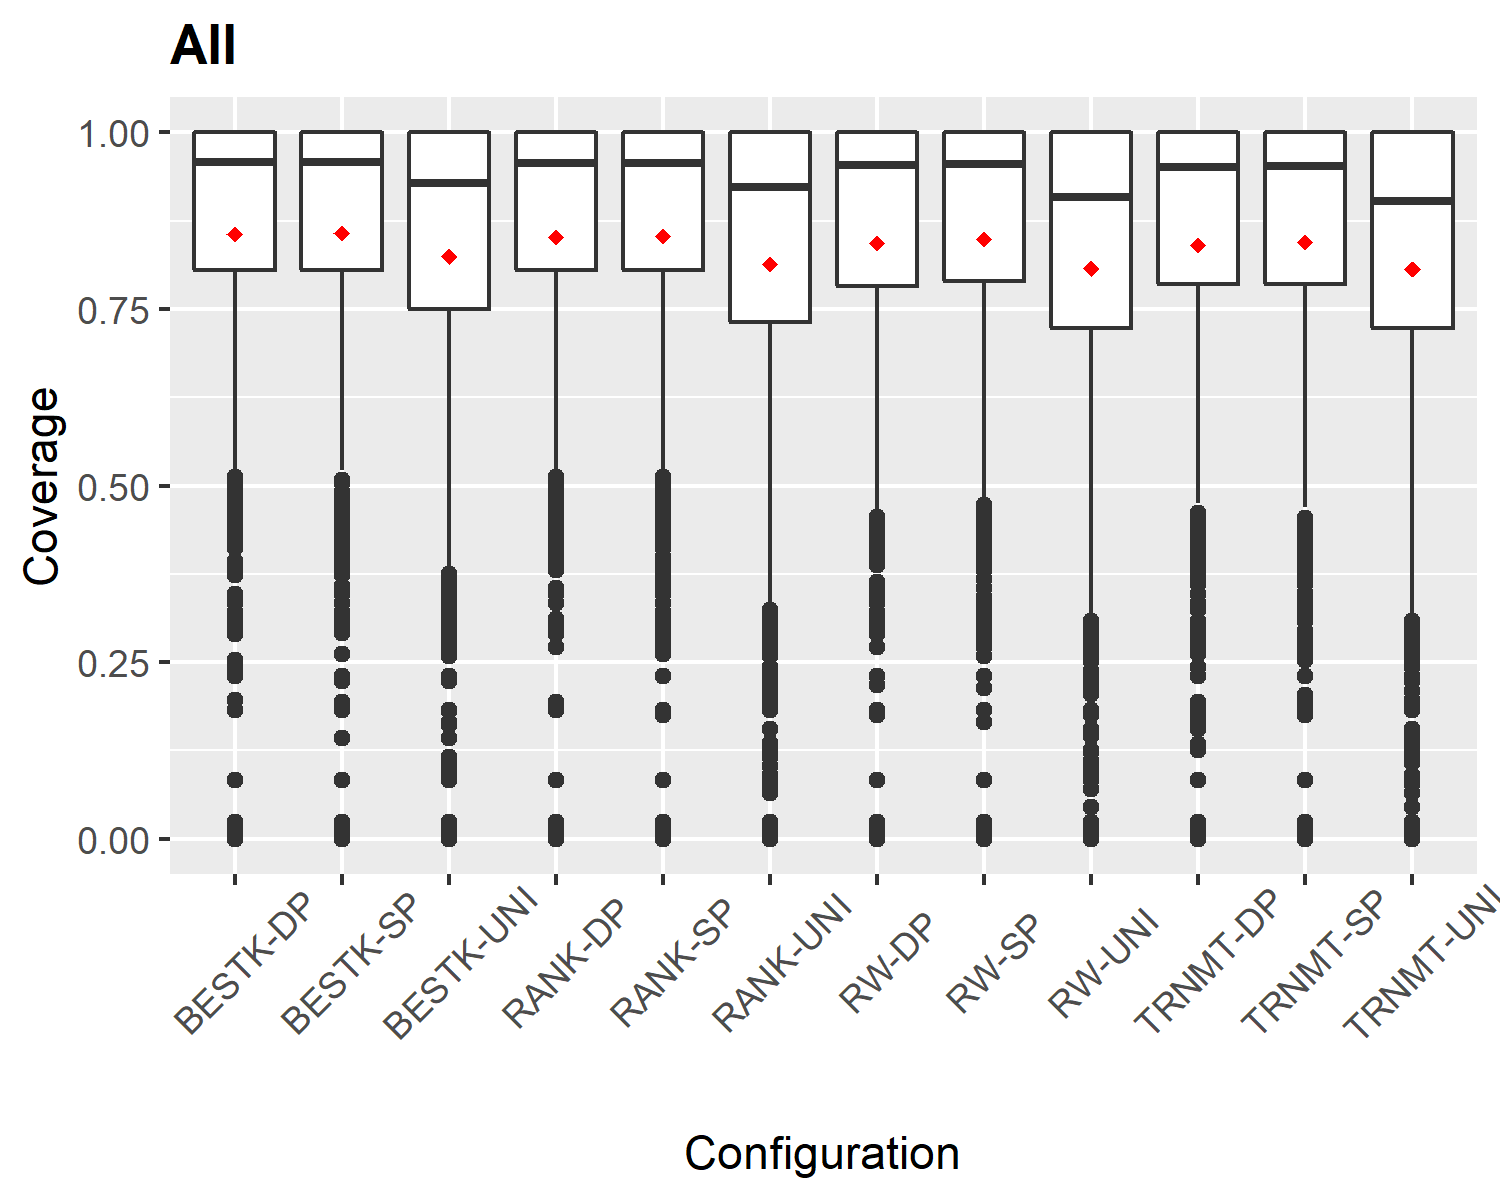
\includegraphics[width=\linewidth]{../output/all-boxplot.png}
  \caption{Box plot of branch coverage across the whole 18,441 tests}
  \Description{Box plot of branch coverage across the whole 18,441 tests}
  \label{fig:allboxplot}
\end{figure}

\subsection{RQ2}
As we observed, the crossover function can impact the branch coverage. The results of Single-point crossover 
and Two-point crossover functions are almost identical. But, the Uniform
crossover function has the worst performance and consistently performs worse than the other two. The highest
average of branch coverage for the Uniform Crossover function was 82.45\%, which is three percent lower than the other two 
crossover functions. Also, the lowest branch coverage for it was 80.69\% when it was used with Tournament Selection
function. It is noticeable that the average count of fitness evaluations of Uniform Crossover function was 
significantly lower than others in all setups. While the average fitness evaluation count of other crossover 
functions was more than 15,000, the highest value for Uniform crossover was 11,655. It is not clear to us that 
whether this observation is due to an implementation bug in EVOSUITE or the nature of Uniform function. 
However, its lower coverage values may be attributed to its algorithm. At each step, the Uniform function mixes 
much more genes than the other two functions, this act may decrease the branch coverage of better individuals.

\subsection{RQ3}
Except for the fact that the Uniform crossover function made results worse, we don't think that choice of 
selection and crossover functions can impact the results. Other factors such as the choice of fitness function and 
the main algorithm (we used the Standard GA) has much more effect as was evaluated by other studies 
\cite{CAMPOS2018207}.

\subsection{Threats to Validity}
We were able to study over a small sample of open-source Java projects and our empirical evaluations are prone 
to External Validity. However, even with our small sample subjects, a few patterns were emerging. 

\section{Conclusion}
\label{conclusion}
To study the effect of several selection and crossover functions on automated test generation with  
Genetic Algorithms, we performed 18,442 tests over 165 Java classes from 10 popular open-source projects. 
We employed the Standard Genetic algorithm implemented in EVOSUITE and measured the impact of 
Uniform, Single-point, and Two-point crossover, and Rank, Tournament, Best-k, Roulette Wheel selection functions.
We discovered that the Uniform crossover function can result in poorer branch coverage. Also, we saw that
the Best-k selection function yields the highest branch coverage. Nevertheless, the impact of various 
selection functions is small and other factors such as fitness function should be configured. 




\begin{figure}[h]
  \centering
  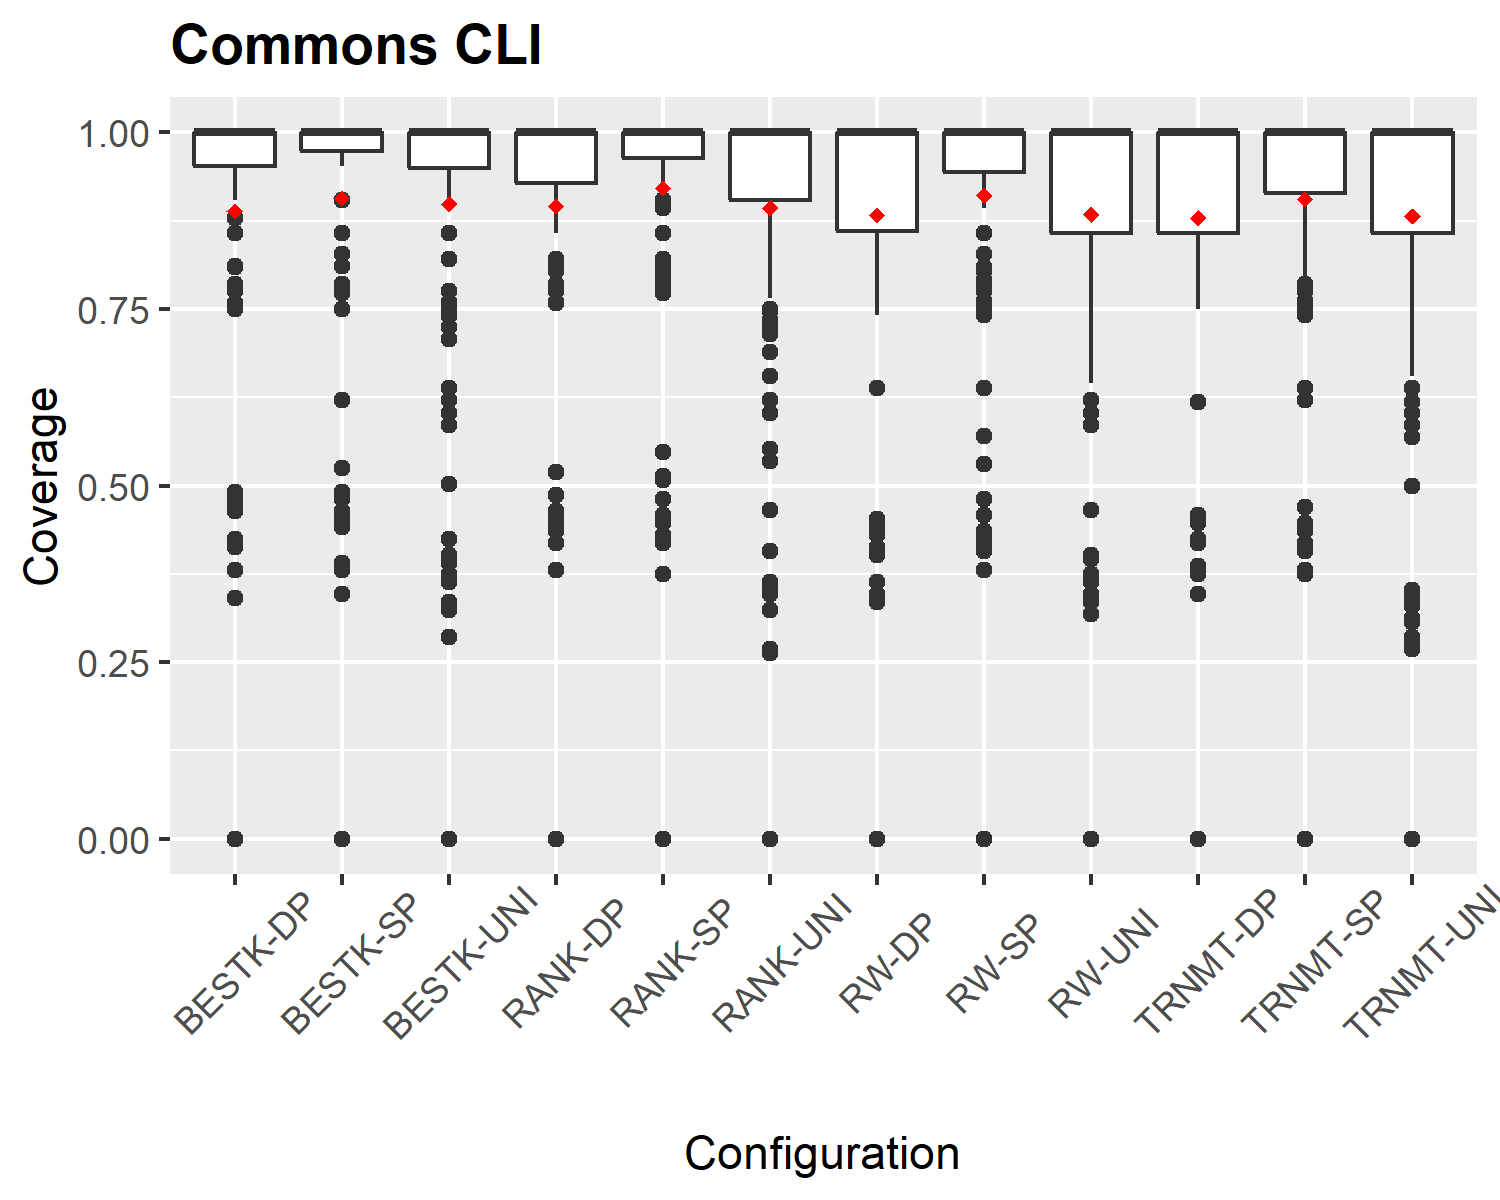
\includegraphics[width=3in]{../output/commons-cli-boxplot.png}
  \caption{Box plot of branch coverage Commons CLI library}
  \Description{Box plot of branch coverage Commons CLI library}
  \label{fig:boxplot1}
\end{figure}

\begin{figure}[h]
  \centering
  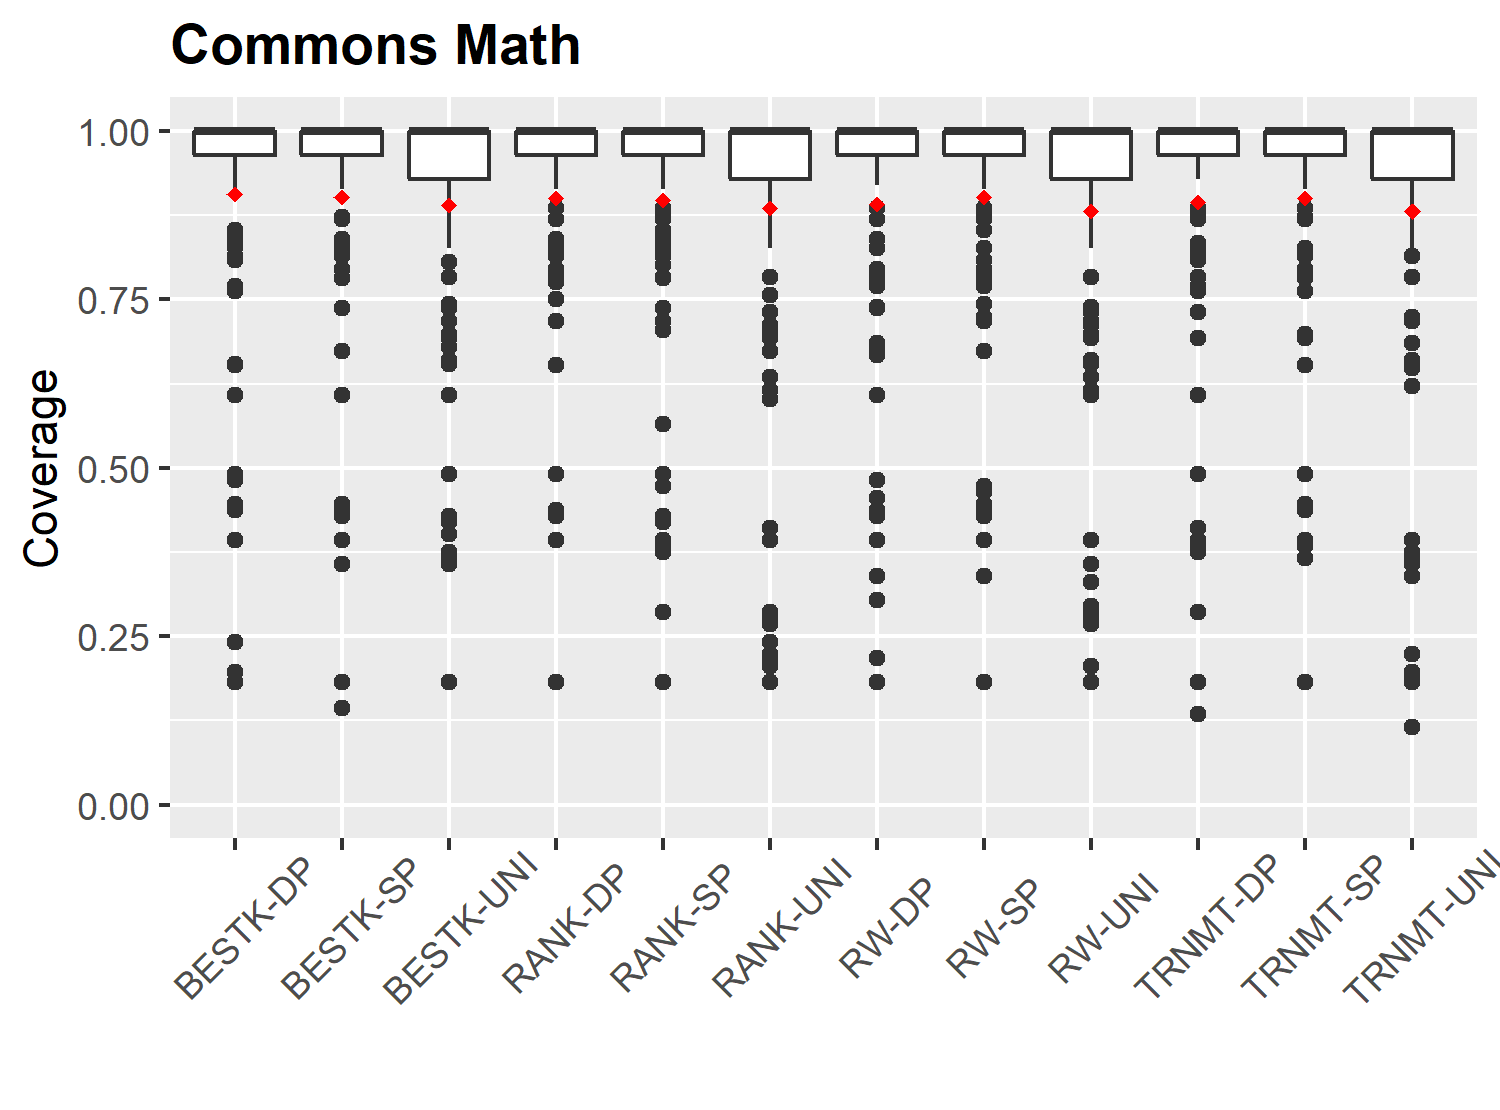
\includegraphics[width=3in]{../output/commons-math-boxplot.png}
  \caption{Box plot of branch coverage Commons Math library}
  \Description{Box plot of branch coverage Commons Math library}
  \label{fig:boxplot2}
\end{figure}

\begin{figure}[h]
  \centering
  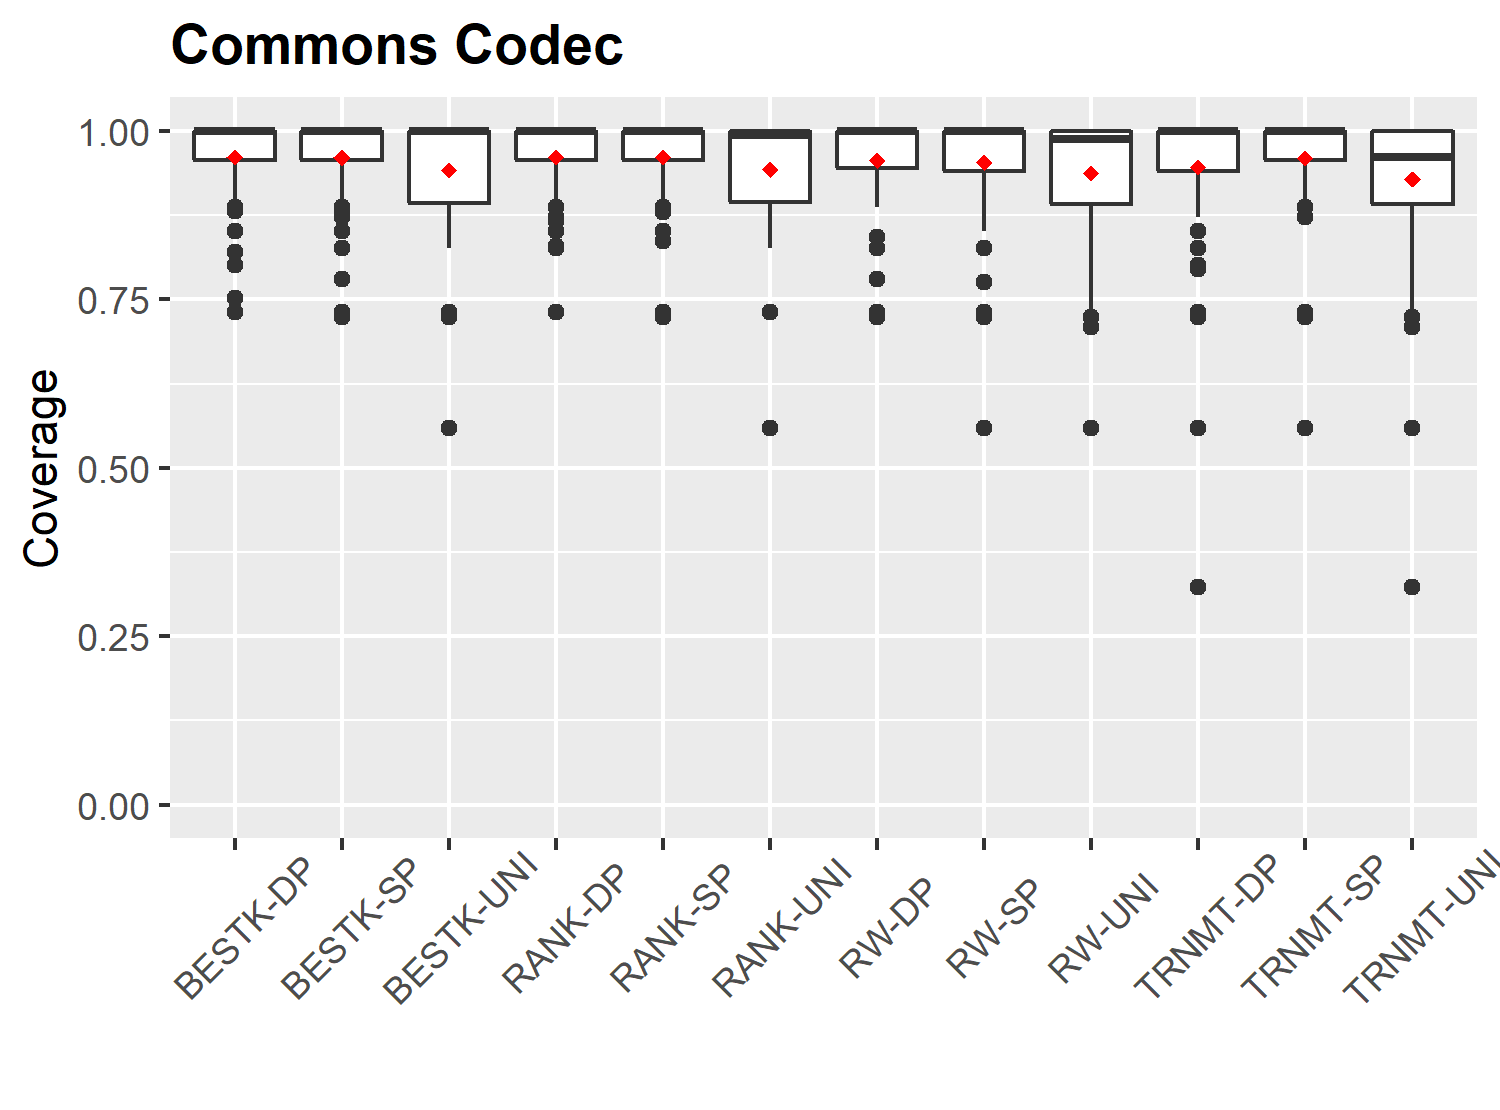
\includegraphics[width=3in]{../output/commons-codec-boxplot.png}
  \caption{Box plot of branch coverage Commons Codec library}
  \Description{Box plot of branch coverage Commons Codec library}
  \label{fig:boxplot3}
\end{figure}

\begin{figure}[h]
  \centering
  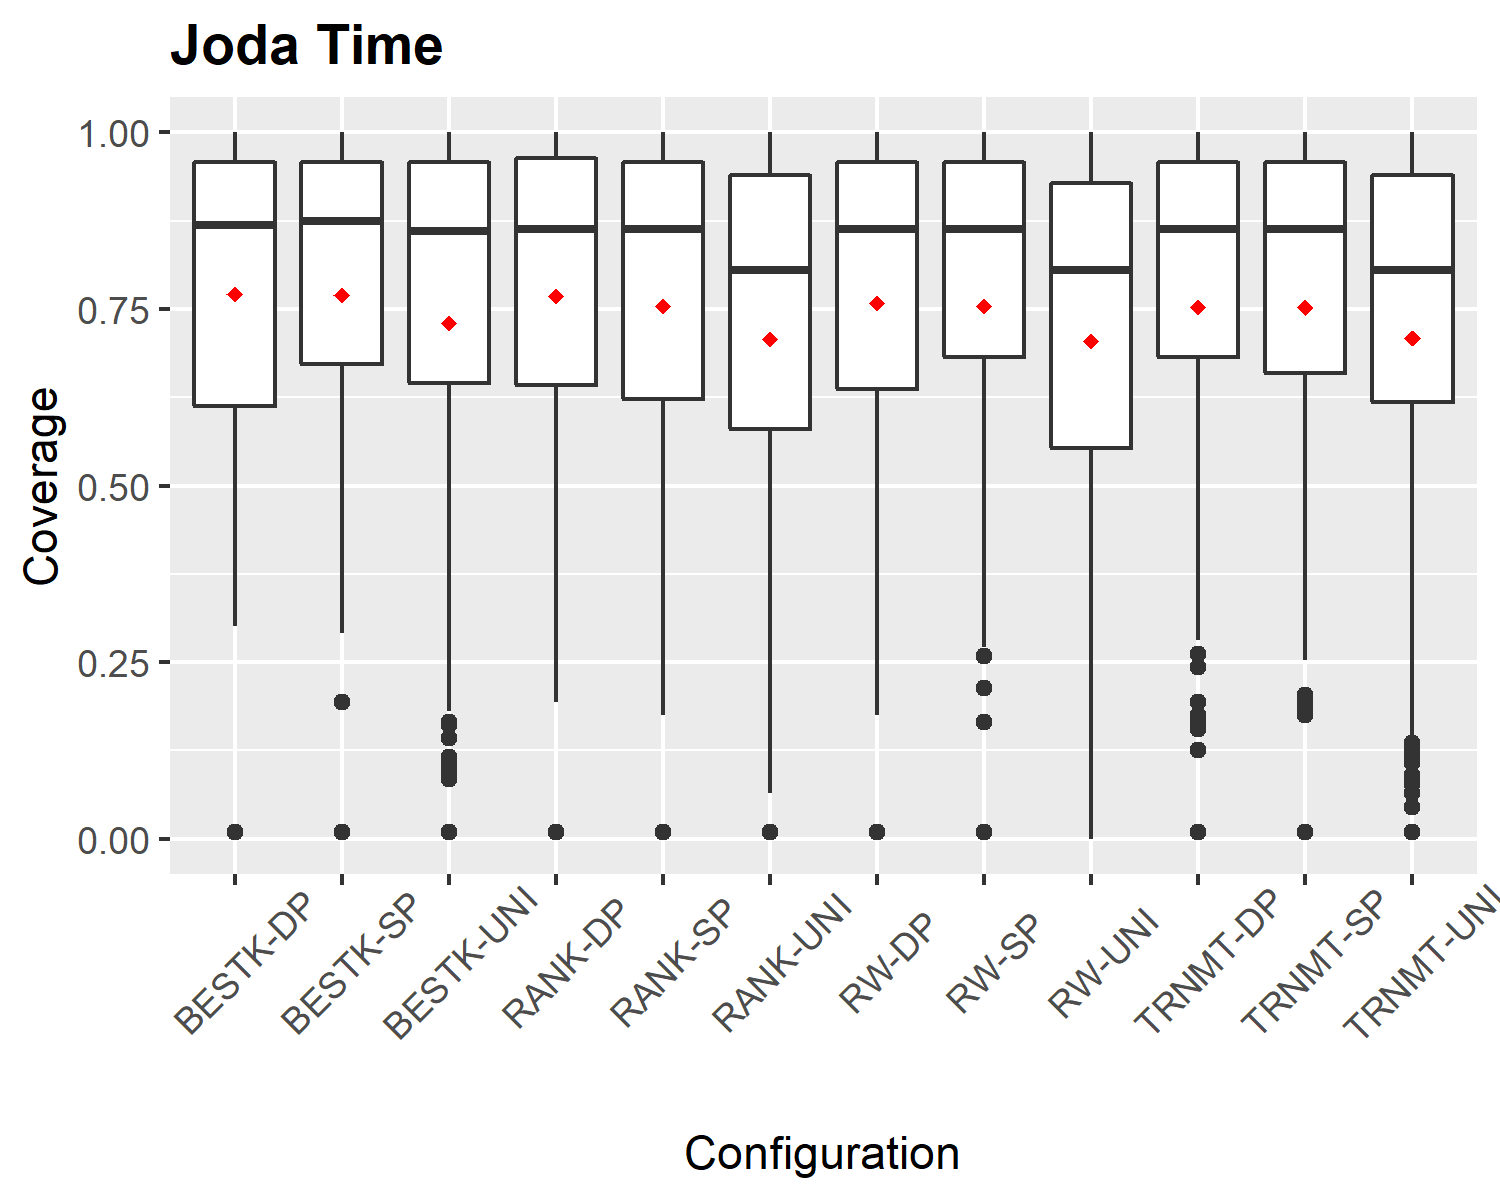
\includegraphics[width=3in]{../output/joda-time-boxplot.png}
  \caption{Box plot of branch coverage Joda Time library}
  \Description{Box plot of branch coverage Joda Time library}
  \label{fig:boxplot4}
\end{figure}

\begin{figure}[h]
  \centering
  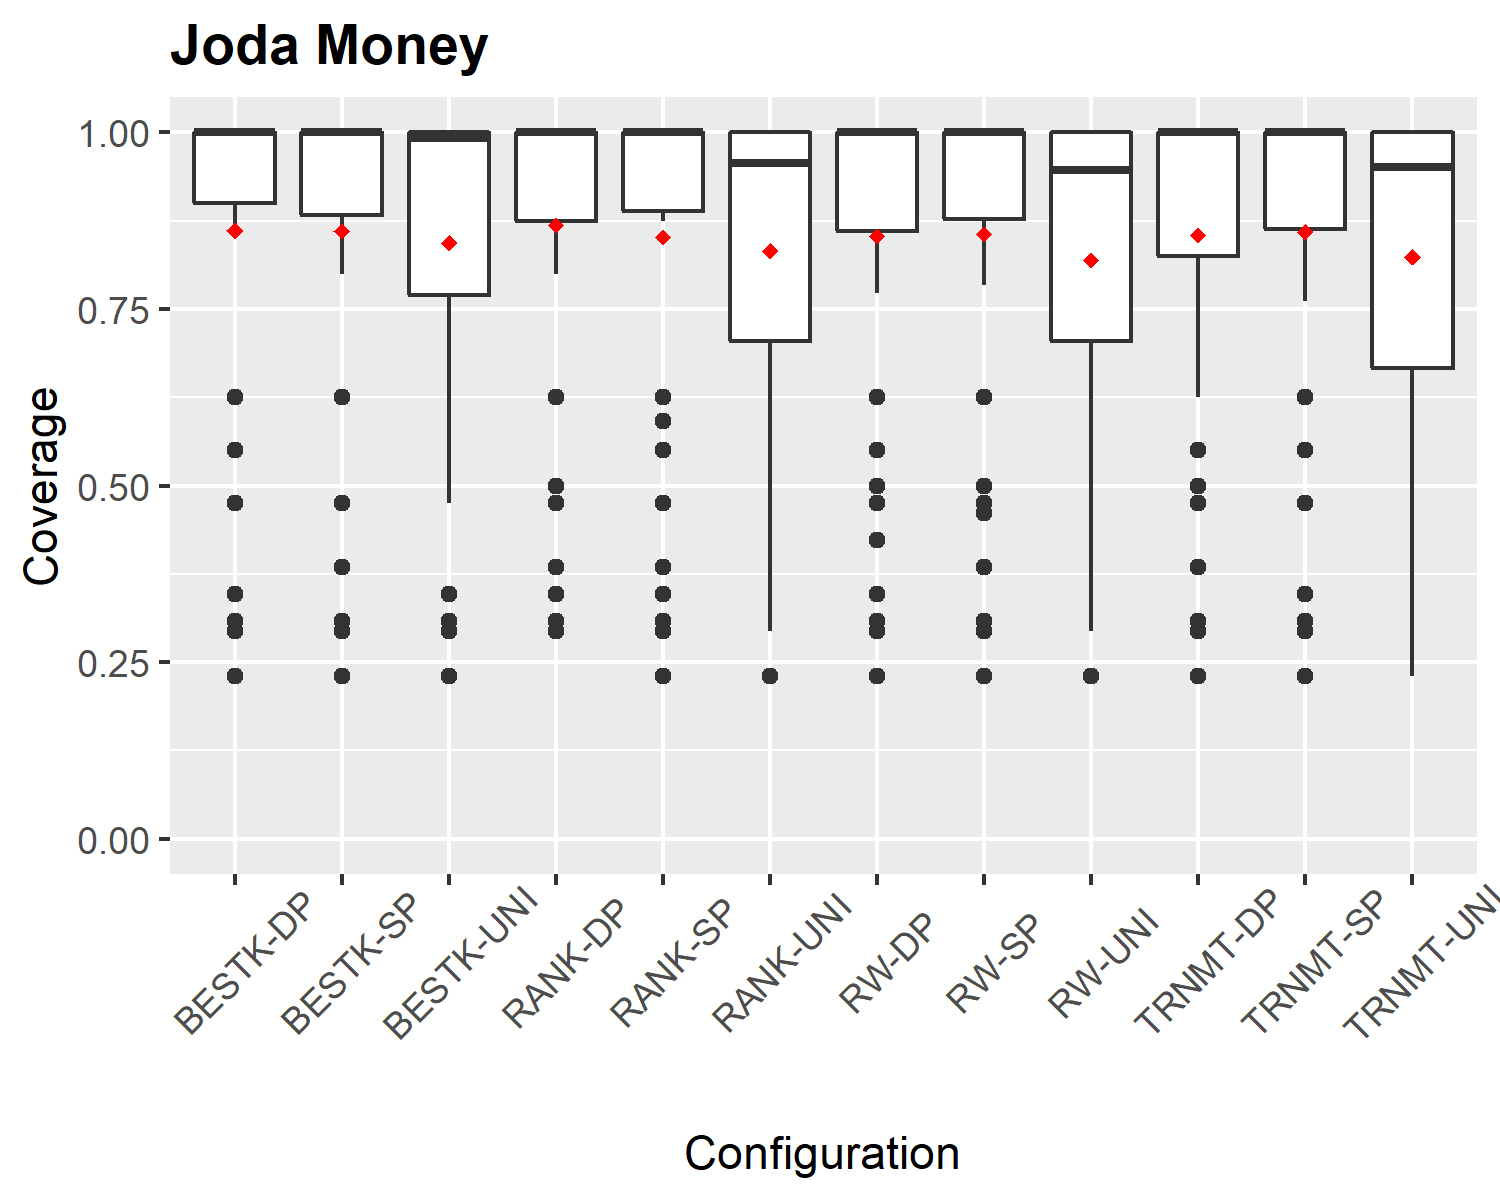
\includegraphics[width=3in]{../output/joda-money-boxplot.png}
  \caption{Box plot of branch coverage Joda Money library}
  \Description{Box plot of branch coverage Joda Money library}
  \label{fig:boxplot5}
\end{figure}

\begin{figure}[h]
  \centering
  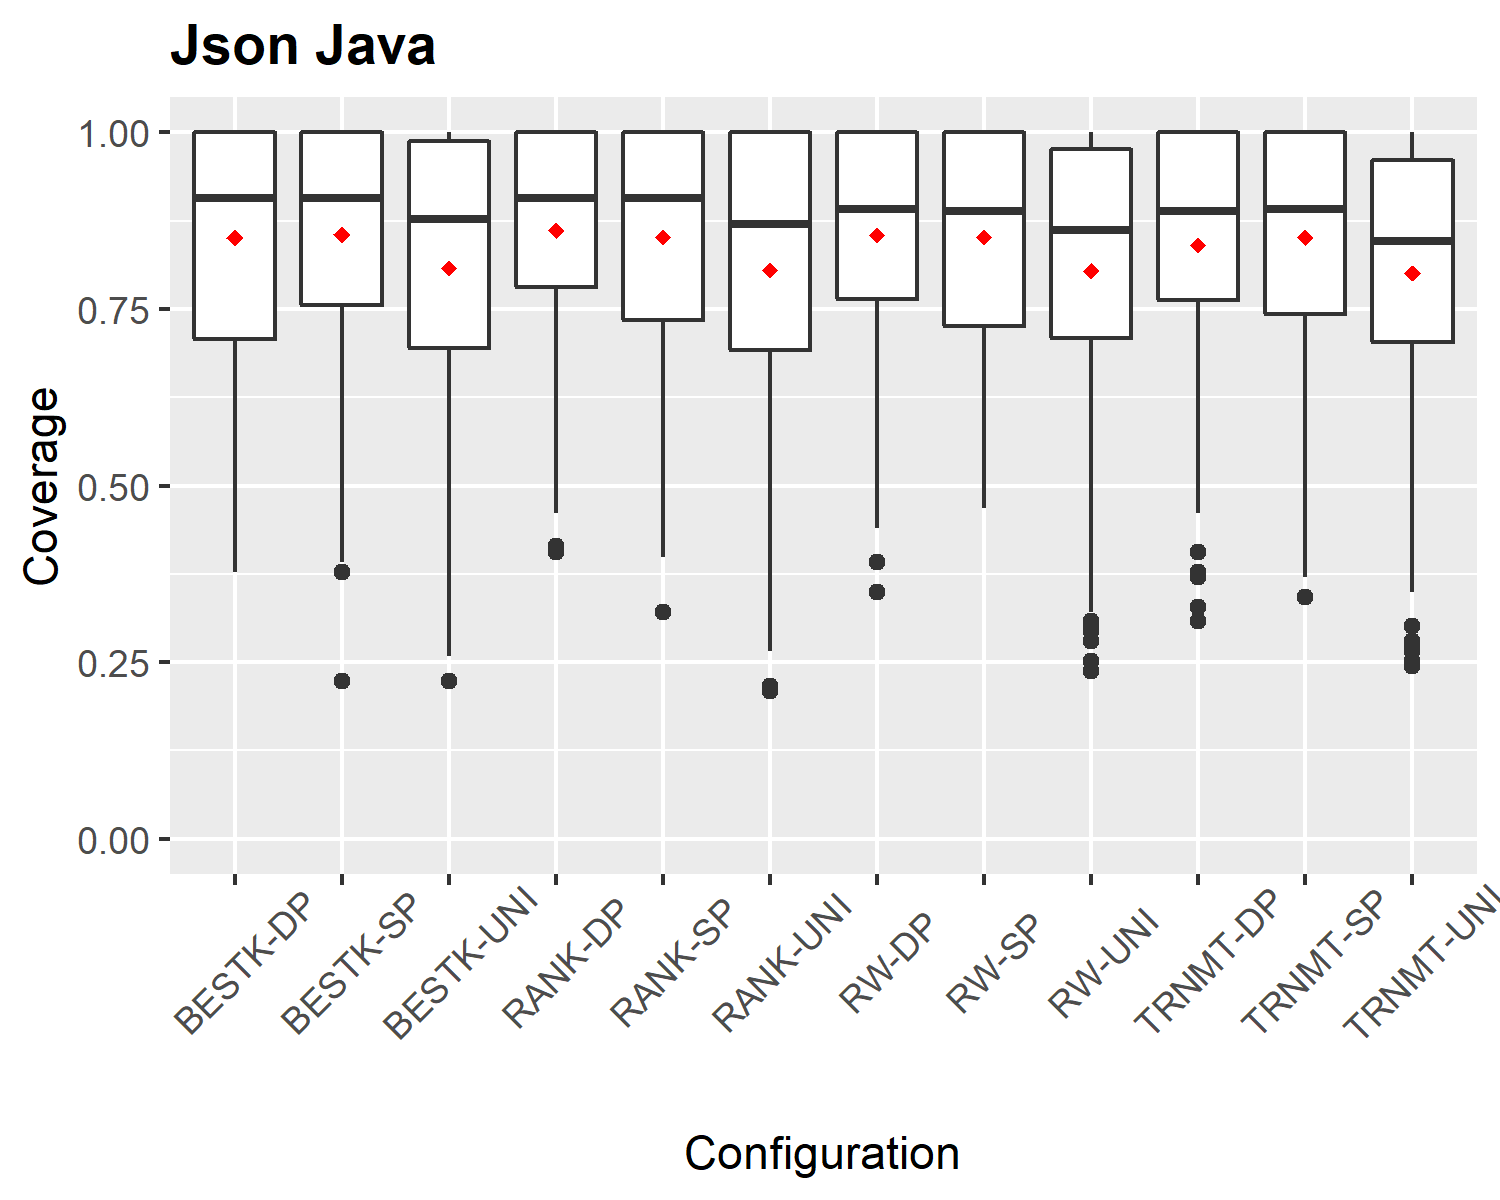
\includegraphics[width=3in]{../output/json-java-boxplot.png}
  \caption{Box plot of branch coverage JSON Java library}
  \Description{Box plot of branch coverage JSON Java library}
  \label{fig:boxplot6}
\end{figure}

\begin{figure}[h]
  \centering
  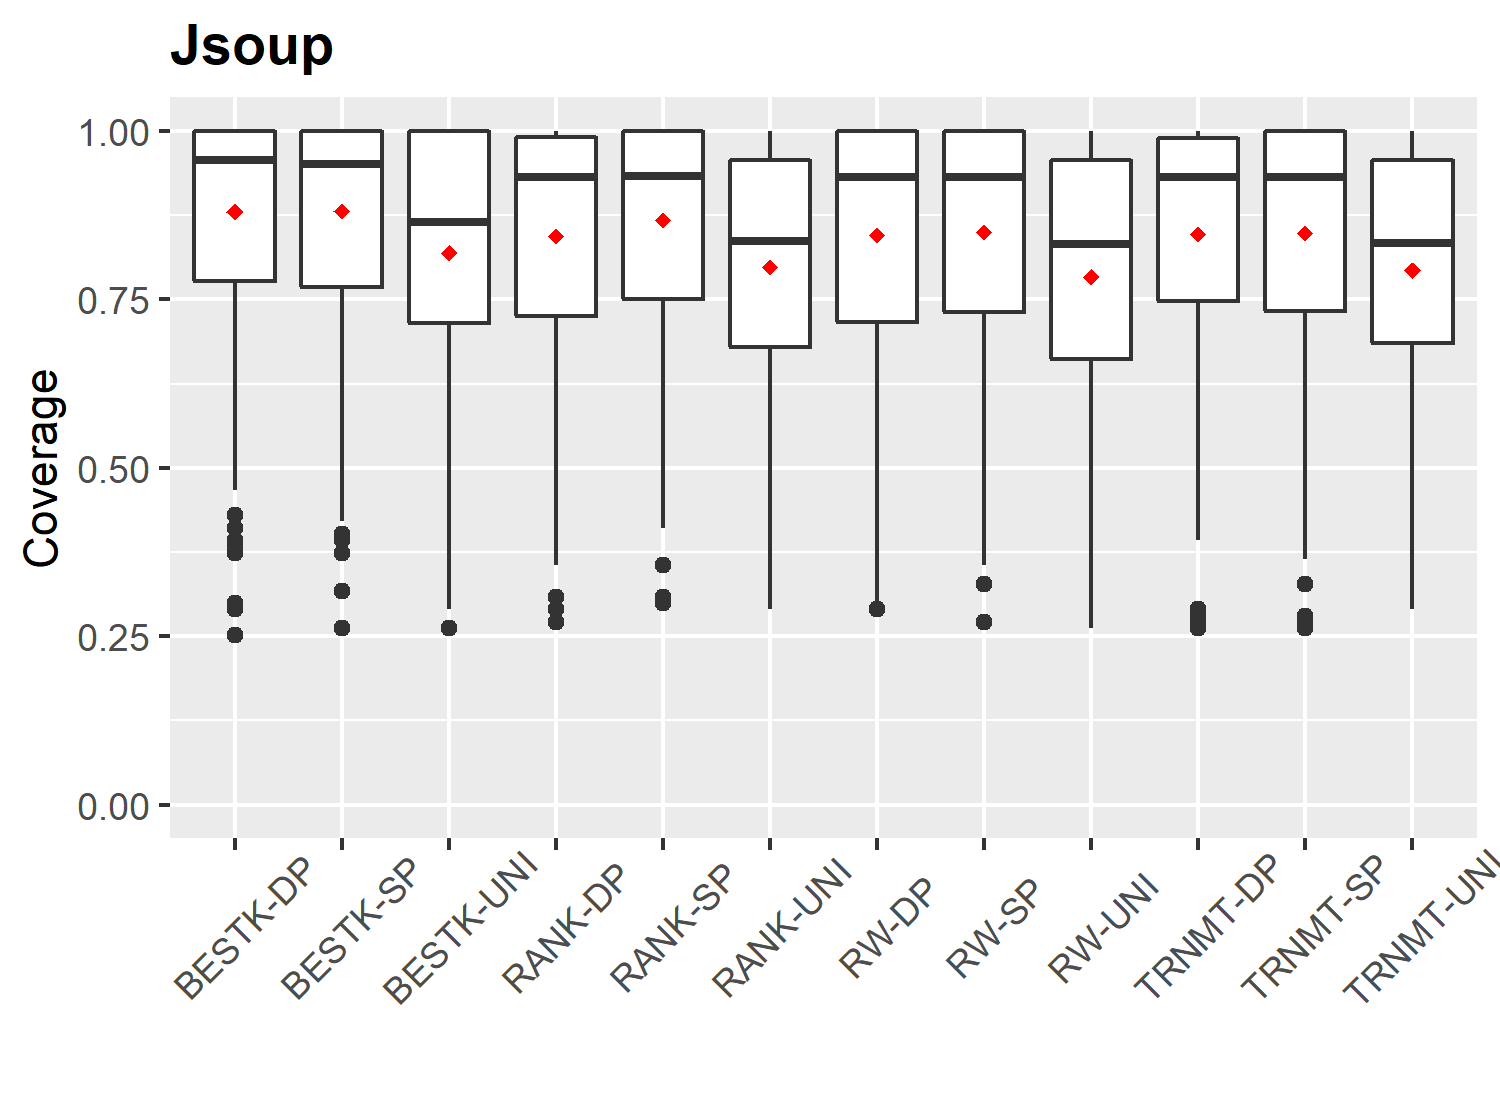
\includegraphics[width=3in]{../output/jsoup-boxplot.png}
  \caption{Box plot of branch coverage Jsoup library}
  \Description{Box plot of branch coverage Jsoup library}
  \label{fig:boxplot7}
\end{figure}

\begin{figure}[h]
  \centering
  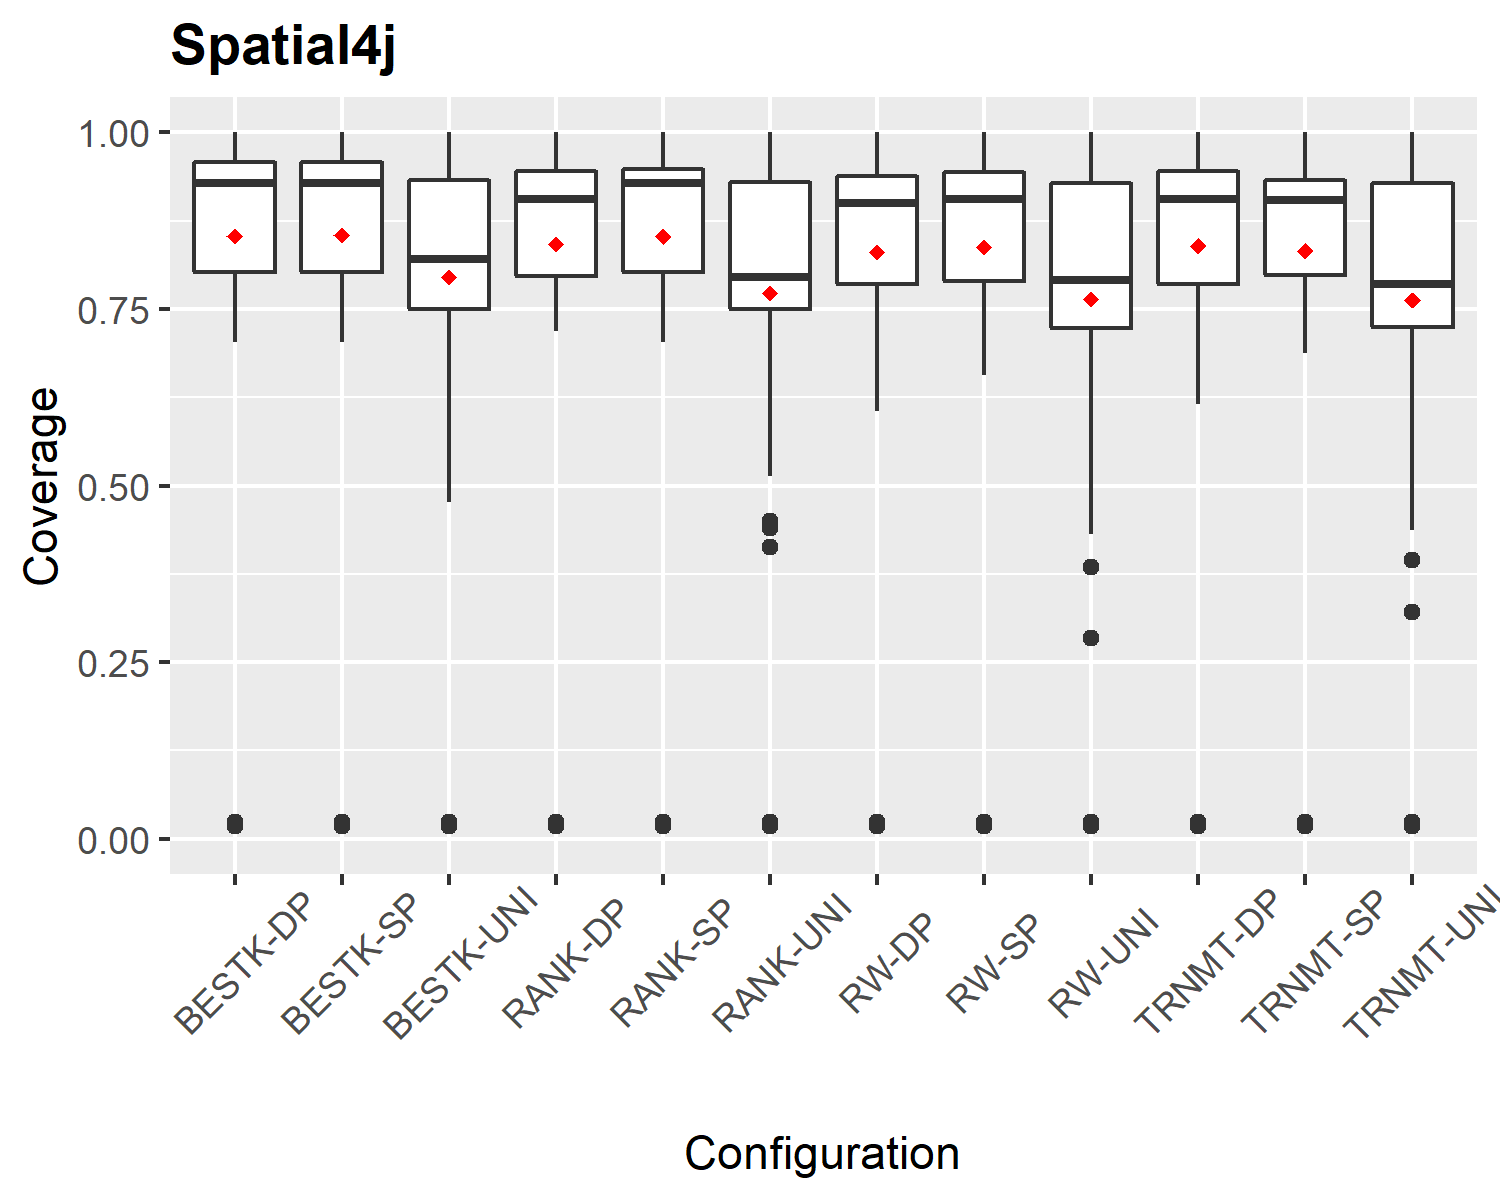
\includegraphics[width=3in]{../output/spatial4j-boxplot.png}
  \caption{Box plot of branch coverage Spatial4j library}
  \Description{Box plot of branch coverage Spatial4j library}
  \label{fig:boxplot8}
\end{figure}

\begin{figure}[h]
  \centering
  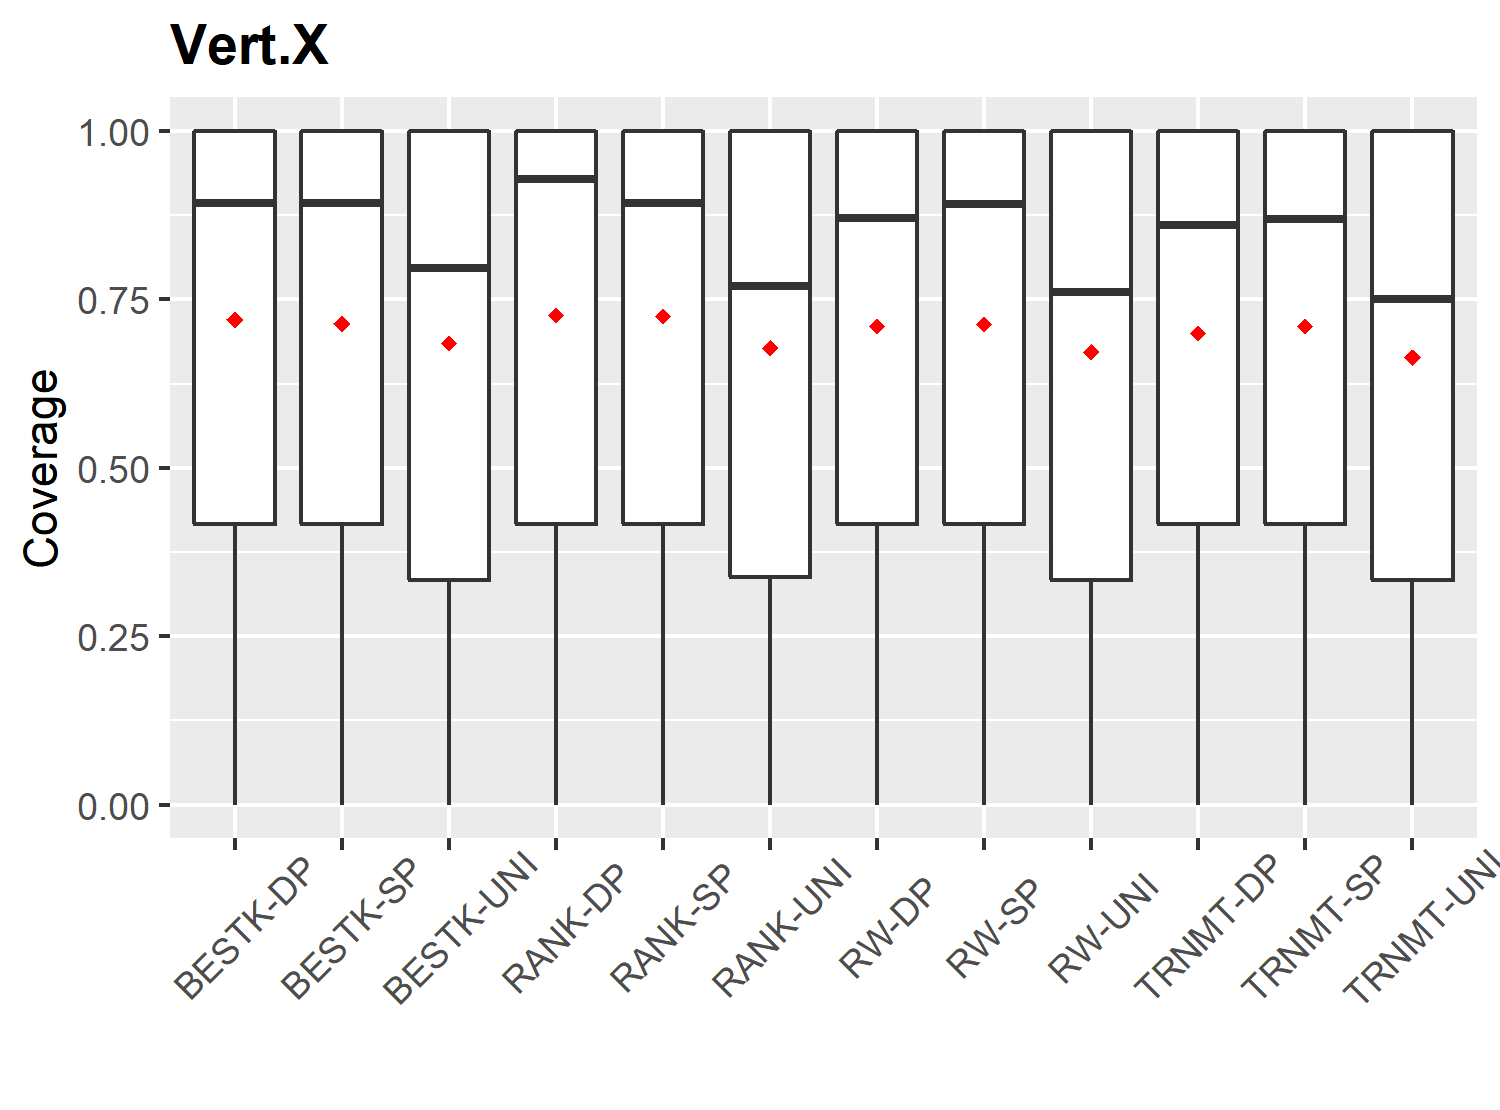
\includegraphics[width=3in]{../output/vertx-boxplot.png}
  \caption{Box plot of branch coverage Vert.x framework}
  \Description{Box plot of branch coverage Vert.x framework}
  \label{fig:boxplot9}
\end{figure}

\begin{figure}[h]
  \centering
  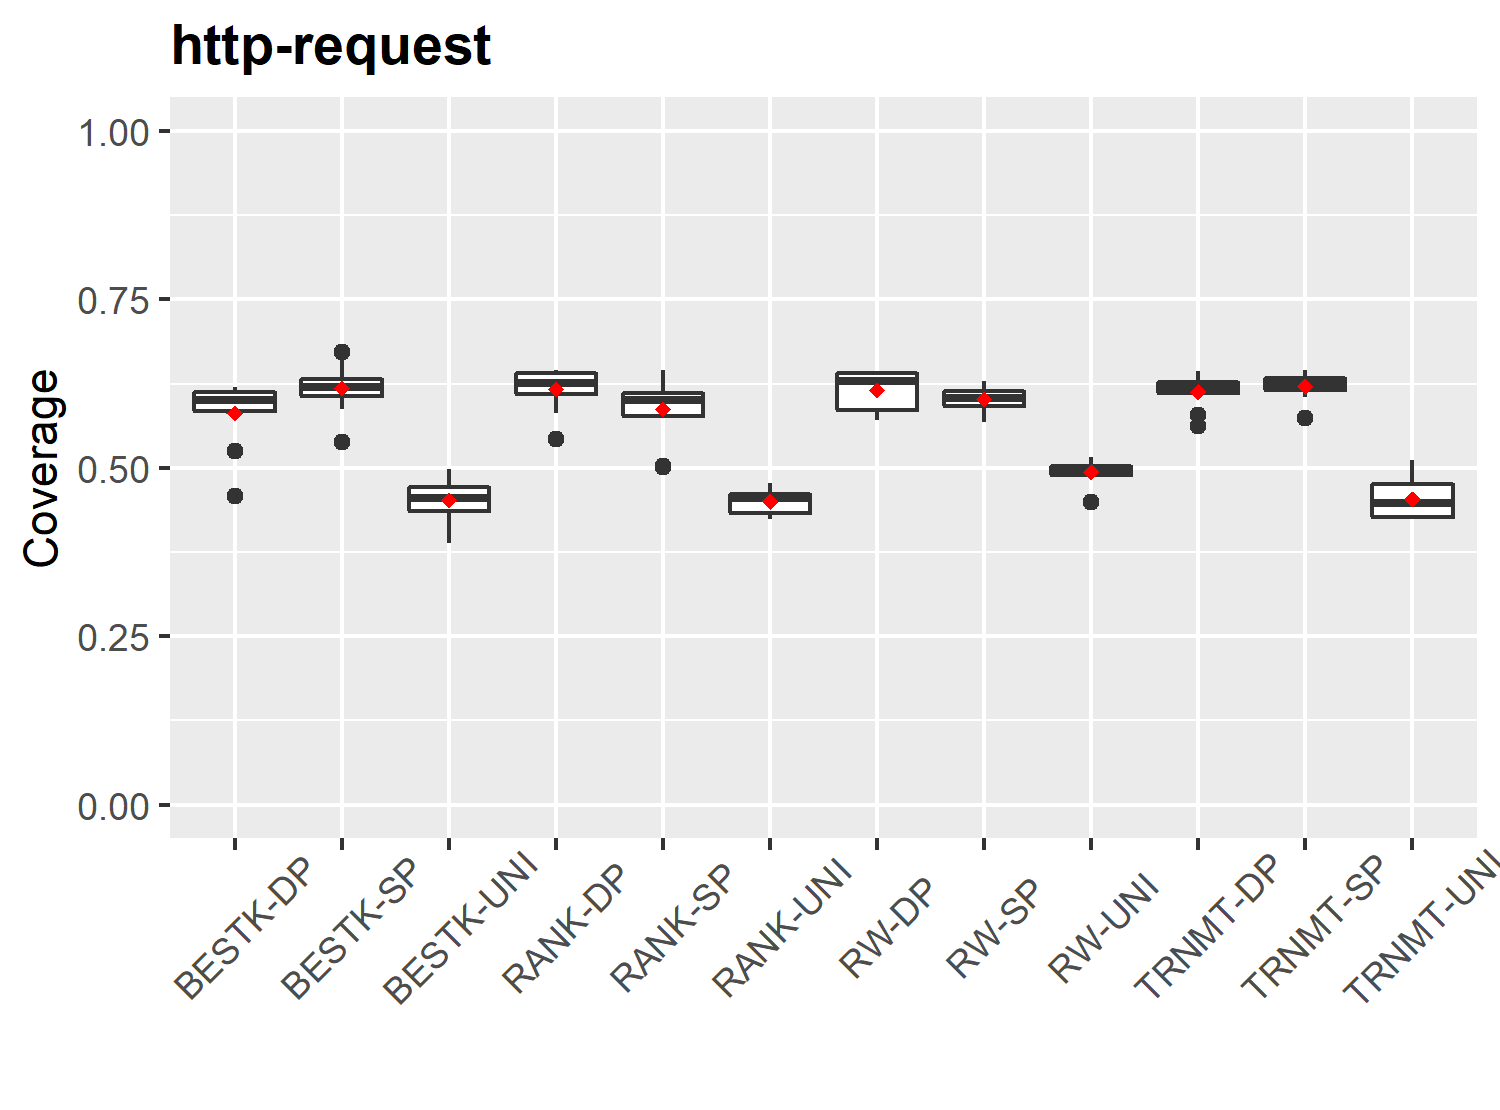
\includegraphics[width=3in]{../output/http-request-boxplot.png}
  \caption{Box plot of branch coverage http-request library}
  \Description{Box plot of branch coverage http-request library}
  \label{fig:boxplot6}
\end{figure}

\clearpage 
\bibliographystyle{ACM-Reference-Format}
\bibliography{citations}

\end{document}
\endinput

% \section{Template Overview}
% As noted in the introduction, the ``\verb|acmart|'' document class can
% be used to prepare many different kinds of documentation --- a
% double-blind initial submission of a full-length technical paper, a
% two-page SIGGRAPH Emerging Technologies abstract, a ``camera-ready''
% journal article, a SIGCHI Extended Abstract, and more --- all by
% selecting the appropriate {\itshape template style} and {\itshape
%   template parameters}.

% This document will explain the major features of the document
% class. For further information, the {\itshape \LaTeX\ User's Guide} is
% available from
% \url{https://www.acm.org/publications/proceedings-template}.

% \subsection{Template Styles}

% The primary parameter given to the ``\verb|acmart|'' document class is
% the {\itshape template style} which corresponds to the kind of publication
% or SIG publishing the work. This parameter is enclosed in square
% brackets and is a part of the {\verb|documentclass|} command:
% \begin{verbatim}
%   \documentclass[STYLE]{acmart}
% \end{verbatim}

% Journals use one of three template styles. All but three ACM journals
% use the {\verb|acmsmall|} template style:
% \begin{itemize}
% \item {\verb|acmsmall|}: The default journal template style.
% \item {\verb|acmlarge|}: Used by JOCCH and TAP.
% \item {\verb|acmtog|}: Used by TOG.
% \end{itemize}

% The majority of conference proceedings documentation will use the {\verb|acmconf|} template style.
% \begin{itemize}
% \item {\verb|acmconf|}: The default proceedings template style.
% \item{\verb|sigchi|}: Used for SIGCHI conference articles.
% \item{\verb|sigchi-a|}: Used for SIGCHI ``Extended Abstract'' articles.
% \item{\verb|sigplan|}: Used for SIGPLAN conference articles.
% \end{itemize}

% \subsection{Template Parameters}

% In addition to specifying the {\itshape template style} to be used in
% formatting your work, there are a number of {\itshape template parameters}
% which modify some part of the applied template style. A complete list
% of these parameters can be found in the {\itshape \LaTeX\ User's Guide.}

% Frequently-used parameters, or combinations of parameters, include:
% \begin{itemize}
% \item {\verb|anonymous,review|}: Suitable for a ``double-blind''
%   conference submission. Anonymizes the work and includes line
%   numbers. Use with the \verb|\acmSubmissionID| command to print the
%   submission's unique ID on each page of the work.
% \item{\verb|authorversion|}: Produces a version of the work suitable
%   for posting by the author.
% \item{\verb|screen|}: Produces colored hyperlinks.
% \end{itemize}

% This document uses the following string as the first command in the
% source file:
% \begin{verbatim}
% \documentclass[sigconf]{acmart}
% \end{verbatim}

% \section{Modifications}

% Modifying the template --- including but not limited to: adjusting
% margins, typeface sizes, line spacing, paragraph and list definitions,
% and the use of the \verb|\vspace| command to manually adjust the
% vertical spacing between elements of your work --- is not allowed.

% {\bfseries Your document will be returned to you for revision if
%   modifications are discovered.}

% \section{Typefaces}

% The ``\verb|acmart|'' document class requires the use of the
% ``Libertine'' typeface family. Your \TeX\ installation should include
% this set of packages. Please do not substitute other typefaces. The
% ``\verb|lmodern|'' and ``\verb|ltimes|'' packages should not be used,
% as they will override the built-in typeface families.

% \section{Title Information}

% The title of your work should use capital letters appropriately -
% \url{https://capitalizemytitle.com/} has useful rules for
% capitalization. Use the {\verb|title|} command to define the title of
% your work. If your work has a subtitle, define it with the
% {\verb|subtitle|} command.  Do not insert line breaks in your title.

% If your title is lengthy, you must define a short version to be used
% in the page headers, to prevent overlapping text. The \verb|title|
% command has a ``short title'' parameter:
% \begin{verbatim}
%   \title[short title]{full title}
% \end{verbatim}

% \section{Authors and Affiliations}

% Each author must be defined separately for accurate metadata
% identification. Multiple authors may share one affiliation. Authors'
% names should not be abbreviated; use full first names wherever
% possible. Include authors' e-mail addresses whenever possible.

% Grouping authors' names or e-mail addresses, or providing an ``e-mail
% alias,'' as shown below, is not acceptable:
% \begin{verbatim}
%   \author{Brooke Aster, David Mehldau}
%   \email{dave,judy,steve@university.edu}
%   \email{firstname.lastname@phillips.org}
% \end{verbatim}

% The \verb|authornote| and \verb|authornotemark| commands allow a note
% to apply to multiple authors --- for example, if the first two authors
% of an article contributed equally to the work.

% If your author list is lengthy, you must define a shortened version of
% the list of authors to be used in the page headers, to prevent
% overlapping text. The following command should be placed just after
% the last \verb|\author{}| definition:
% \begin{verbatim}
%   \renewcommand{\shortauthors}{McCartney, et al.}
% \end{verbatim}
% Omitting this command will force the use of a concatenated list of all
% of the authors' names, which may result in overlapping text in the
% page headers.

% The article template's documentation, available at
% \url{https://www.acm.org/publications/proceedings-template}, has a
% complete explanation of these commands and tips for their effective
% use.

% Note that authors' addresses are mandatory for journal articles.

% \section{Rights Information}

% Authors of any work published by ACM will need to complete a rights
% form. Depending on the kind of work, and the rights management choice
% made by the author, this may be copyright transfer, permission,
% license, or an OA (open access) agreement.

% Regardless of the rights management choice, the author will receive a
% copy of the completed rights form once it has been submitted. This
% form contains \LaTeX\ commands that must be copied into the source
% document. When the document source is compiled, these commands and
% their parameters add formatted text to several areas of the final
% document:
% \begin{itemize}
% \item the ``ACM Reference Format'' text on the first page.
% \item the ``rights management'' text on the first page.
% \item the conference information in the page header(s).
% \end{itemize}

% Rights information is unique to the work; if you are preparing several
% works for an event, make sure to use the correct set of commands with
% each of the works.

% The ACM Reference Format text is required for all articles over one
% page in length, and is optional for one-page articles (abstracts).

% \section{CCS Concepts and User-Defined Keywords}

% Two elements of the ``acmart'' document class provide powerful
% taxonomic tools for you to help readers find your work in an online
% search.

% The ACM Computing Classification System ---
% \url{https://www.acm.org/publications/class-2012} --- is a set of
% classifiers and concepts that describe the computing
% discipline. Authors can select entries from this classification
% system, via \url{https://dl.acm.org/ccs/ccs.cfm}, and generate the
% commands to be included in the \LaTeX\ source.

% User-defined keywords are a comma-separated list of words and phrases
% of the authors' choosing, providing a more flexible way of describing
% the research being presented.

% CCS concepts and user-defined keywords are required for for all
% articles over two pages in length, and are optional for one- and
% two-page articles (or abstracts).

% \section{Sectioning Commands}

% Your work should use standard \LaTeX\ sectioning commands:
% \verb|section|, \verb|subsection|, \verb|subsubsection|, and
% \verb|paragraph|. They should be numbered; do not remove the numbering
% from the commands.

% Simulating a sectioning command by setting the first word or words of
% a paragraph in boldface or italicized text is {\bfseries not allowed.}

% \section{Tables}

% The ``\verb|acmart|'' document class includes the ``\verb|booktabs|''
% package --- \url{https://ctan.org/pkg/booktabs} --- for preparing
% high-quality tables.

% Table captions are placed {\itshape above} the table.

% Because tables cannot be split across pages, the best placement for
% them is typically the top of the page nearest their initial cite.  To
% ensure this proper ``floating'' placement of tables, use the
% environment \textbf{table} to enclose the table's contents and the
% table caption.  The contents of the table itself must go in the
% \textbf{tabular} environment, to be aligned properly in rows and
% columns, with the desired horizontal and vertical rules.  Again,
% detailed instructions on \textbf{tabular} material are found in the
% \textit{\LaTeX\ User's Guide}.

% Immediately following this sentence is the point at which
% Table~\ref{tab:freq} is included in the input file; compare the
% placement of the table here with the table in the printed output of
% this document.

% \begin{table}
%   \caption{Frequency of Special Characters}
%   \label{tab:freq}
%   \begin{tabular}{ccl}
%     \toprule
%     Non-English or Math & Frequency & Comments\\
%     \midrule
%     $\sigma$ & 1 inasc 1,000 & For Swedish names\\
%     $\pi$ & 1 in 5 & Common in math\\
%     \$ & 4 in 5 & Used in business\\
%     $\Psi^2_1$ & 1 in 40,000 & Unexplained usage\\
%   \bottomrule
% \end{tabular}
% \end{table}

% To set a wider table, which takes up the whole width of the page's
% live area, use the environment \textbf{table*} to enclose the table's
% contents and the table caption.  As with a single-column table, this
% wide table will ``float'' to a location deemed more
% desirable. Immediately following this sentence is the point at which
% Table~\ref{tab:commands} is included in the input file; again, it is
% instructive to compare the placement of the table here with the table
% in the printed output of this document.

% \begin{table*}
%   \caption{Some Typical Commands}
%   \label{tab:commands}
%   \begin{tabular}{ccl}
%     \toprule
%     Command &A Number & Comments\\
%     \midrule
%     \texttt{{\char'134}author} & 100& Author \\
%     \texttt{{\char'134}table}& 300 & For tables\\
%     \texttt{{\char'134}table*}& 400& For wider tables\\
%     \bottomrule
%   \end{tabular}
% \end{table*}

% Always use midrule to separate table header rows from data rows, and
% use it only for this purpose. This enables assistive technologies to
% recognise table headers and support their users in navigating tables
% more easily.

% \section{Math Equations}
% You may want to display math equations in three distinct styles:
% inline, numbered or non-numbered display.  Each of the three are
% discussed in the next sections.

% \subsection{Inline (In-text) Equations}
% A formula that appears in the running text is called an inline or
% in-text formula.  It is produced by the \textbf{math} environment,
% which can be invoked with the usual
% \texttt{{\char'134}begin\,\ldots{\char'134}end} construction or with
% the short form \texttt{\$\,\ldots\$}. You can use any of the symbols
% and structures, from $\alpha$ to $\omega$, available in
% \LaTeX~\cite{Lamport:LaTeX}; this section will simply show a few
% examples of in-text equations in context. Notice how this equation:
% \begin{math}
%   \lim_{n\rightarrow \infty}x=0
% \end{math},
% set here in in-line math style, looks slightly different when
% set in display style.  (See next section).

% \subsection{Display Equations}
% A numbered display equation---one set off by vertical space from the
% text and centered horizontally---is produced by the \textbf{equation}
% environment. An unnumbered display equation is produced by the
% \textbf{displaymath} environment.

% Again, in either environment, you can use any of the symbols and
% structures available in \LaTeX\@; this section will just give a couple
% of examples of display equations in context.  First, consider the
% equation, shown as an inline equation above:
% \begin{equation}
%   \lim_{n\rightarrow \infty}x=0
% \end{equation}
% Notice how it is formatted somewhat differently in
% the \textbf{displaymath}
% environment.  Now, we'll enter an unnumbered equation:
% \begin{displaymath}
%   \sum_{i=0}^{\infty} x + 1
% \end{displaymath}
% and follow it with another numbered equation:
% \begin{equation}
%   \sum_{i=0}^{\infty}x_i=\int_{0}^{\pi+2} f
% \end{equation}
% just to demonstrate \LaTeX's able handling of numbering.

% \section{Figures}

% The ``\verb|figure|'' environment should be used for figures. One or
% more images can be placed within a figure. If your figure contains
% third-party material, you must clearly identify it as such, as shown
% in the example below.
% \begin{figure}[h]
%   \centering
%   \includegraphics[width=\linewidth]{sample-franklin}
%   \caption{1907 Franklin Model D roadster. Photograph by Harris \&
%     Ewing, Inc. [Public domain], via Wikimedia
%     Commons. (\url{https://goo.gl/VLCRBB}).}
%   \Description{A woman and a girl in white dresses sit in an open car.}
% \end{figure}

% Your figures should contain a caption which describes the figure to
% the reader.

% Figure captions are placed {\itshape below} the figure.

% Every figure should also have a figure description unless it is purely
% decorative. These descriptions convey what’s in the image to someone
% who cannot see it. They are also used by search engine crawlers for
% indexing images, and when images cannot be loaded.

% A figure description must be unformatted plain text less than 2000
% characters long (including spaces).  {\bfseries Figure descriptions
%   should not repeat the figure caption – their purpose is to capture
%   important information that is not already provided in the caption or
%   the main text of the paper.} For figures that convey important and
% complex new information, a short text description may not be
% adequate. More complex alternative descriptions can be placed in an
% appendix and referenced in a short figure description. For example,
% provide a data table capturing the information in a bar chart, or a
% structured list representing a graph.  For additional information
% regarding how best to write figure descriptions and why doing this is
% so important, please see
% \url{https://www.acm.org/publications/taps/describing-figures/}.

% \subsection{The ``Teaser Figure''}

% A ``teaser figure'' is an image, or set of images in one figure, that
% are placed after all author and affiliation information, and before
% the body of the article, spanning the page. If you wish to have such a
% figure in your article, place the command immediately before the
% \verb|\maketitle| command:
% \begin{verbatim}
%   \begin{teaserfigure}
%     \includegraphics[width=\textwidth]{sampleteaser}
%     \caption{figure caption}
%     \Description{figure description}
%   \end{teaserfigure}
% \end{verbatim}

% \section{Citations and Bibliographies}

% The use of \BibTeX\ for the preparation and formatting of one's
% references is strongly recommended. Authors' names should be complete
% --- use full first names (``Donald E. Knuth'') not initials
% (``D. E. Knuth'') --- and the salient identifying features of a
% reference should be included: title, year, volume, number, pages,
% article DOI, etc.

% The bibliography is included in your source document with these two
% commands, placed just before the \verb|\end{document}| command:
% \begin{verbatim}
%   \bibliographystyle{ACM-Reference-Format}
%   \bibliography{bibfile}
% \end{verbatim}
% where ``\verb|bibfile|'' is the name, without the ``\verb|.bib|''
% suffix, of the \BibTeX\ file.

% Citations and references are numbered by default. A small number of
% ACM publications have citations and references formatted in the
% ``author year'' style; for these exceptions, please include this
% command in the {\bfseries preamble} (before the command
% ``\verb|\begin{document}|'') of your \LaTeX\ source:
% \begin{verbatim}
%   \citestyle{acmauthoryear}
% \end{verbatim}

%   Some examples.  A paginated journal article \cite{Abril07}, an
%   enumerated journal article \cite{Cohen07}, a reference to an entire
%   issue \cite{JCohen96}, a monograph (whole book) \cite{Kosiur01}, a
%   monograph/whole book in a series (see 2a in spec. document)
%   \cite{Harel79}, a divisible-book such as an anthology or compilation
%   \cite{Editor00} followed by the same example, however we only output
%   the series if the volume number is given \cite{Editor00a} (so
%   Editor00a's series should NOT be present since it has no vol. no.),
%   a chapter in a divisible book \cite{Spector90}, a chapter in a
%   divisible book in a series \cite{Douglass98}, a multi-volume work as
%   book \cite{Knuth97}, a couple of articles in a proceedings (of a
%   conference, symposium, workshop for example) (paginated proceedings
%   article) \cite{Andler79, Hagerup1993}, a proceedings article with
%   all possible elements \cite{Smith10}, an example of an enumerated
%   proceedings article \cite{VanGundy07}, an informally published work
%   \cite{Harel78}, a couple of preprints \cite{Bornmann2019,
%     AnzarootPBM14}, a doctoral dissertation \cite{Clarkson85}, a
%   master's thesis: \cite{anisi03}, an online document / world wide web
%   resource \cite{Thornburg01, Ablamowicz07, Poker06}, a video game
%   (Case 1) \cite{Obama08} and (Case 2) \cite{Novak03} and \cite{Lee05}
%   and (Case 3) a patent \cite{JoeScientist001}, work accepted for
%   publication \cite{rous08}, 'YYYYb'-test for prolific author
%   \cite{SaeediMEJ10} and \cite{SaeediJETC10}. Other cites might
%   contain 'duplicate' DOI and URLs (some SIAM articles)
%   \cite{Kirschmer:2010:AEI:1958016.1958018}. Boris / Barbara Beeton:
%   multi-volume works as books \cite{MR781536} and \cite{MR781537}. A
%   couple of citations with DOIs:
%   \cite{2004:ITE:1009386.1010128,Kirschmer:2010:AEI:1958016.1958018}. Online
%   citations: \cite{TUGInstmem, Thornburg01, CTANacmart}. Artifacts:
%   \cite{R} and \cite{UMassCitations}.

% \section{Acknowledgments}

% Identification of funding sources and other support, and thanks to
% individuals and groups that assisted in the research and the
% preparation of the work should be included in an acknowledgment
% section, which is placed just before the reference section in your
% document.

% This section has a special environment:
% \begin{verbatim}
%   \begin{acks}
%   ...
%   \end{acks}
% \end{verbatim}
% so that the information contained therein can be more easily collected
% during the article metadata extraction phase, and to ensure
% consistency in the spelling of the section heading.

% Authors should not prepare this section as a numbered or unnumbered {\verb|\section|}; please use the ``{\verb|acks|}'' environment.

% \section{Appendices}

% If your work needs an appendix, add it before the
% ``\verb|\end{document}|'' command at the conclusion of your source
% document.

% Start the appendix with the ``\verb|appendix|'' command:
% \begin{verbatim}
%   \appendix
% \end{verbatim}
% and note that in the appendix, sections are lettered, not
% numbered. This document has two appendices, demonstrating the section
% and subsection identification method.

% \section{SIGCHI Extended Abstracts}

% The ``\verb|sigchi-a|'' template style (available only in \LaTeX\ and
% not in Word) produces a landscape-orientation formatted article, with
% a wide left margin. Three environments are available for use with the
% ``\verb|sigchi-a|'' template style, and produce formatted output in
% the margin:
% \begin{itemize}
% \item {\verb|sidebar|}:  Place formatted text in the margin.
% \item {\verb|marginfigure|}: Place a figure in the margin.
% \item {\verb|margintable|}: Place a table in the margin.
% \end{itemize}

%%
%% The acknowledgments section is defined using the "acks" environment
%% (and NOT an unnumbered section). This ensures the proper
%% identification of the section in the article metadata, and the
%% consistent spelling of the heading.
% \begin{acks}
% To Robert, for the bagels and explaining CMYK and color spaces.
% \end{acks}

%%
%% The next two lines define the bibliography style to be used, and
%% the bibliography file.

%%
%% If your work has an appendix, this is the place to put it.
% \appendix

% \section{Research Methods}

% \subsection{Part One}

% Lorem ipsum dolor sit amet, consectetur adipiscing elit. Morbi
% malesuada, quam in pulvinar varius, metus nunc fermentum urna, id
% sollicitudin purus odio sit amet enim. Aliquam ullamcorper eu ipsum
% vel mollis. Curabitur quis dictum nisl. Phasellus vel semper risus, et
% lacinia dolor. Integer ultricies commodo sem nec semper.

% \subsection{Part Two}

% Etiam commodo feugiat nisl pulvinar pellentesque. Etiam auctor sodales
% ligula, non varius nibh pulvinar semper. Suspendisse nec lectus non
% ipsum convallis congue hendrerit vitae sapien. Donec at laoreet
% eros. Vivamus non purus placerat, scelerisque diam eu, cursus
% ante. Etiam aliquam tortor auctor efficitur mattis.

% \section{Online Resources}

% Nam id fermentum dui. Suspendisse sagittis tortor a nulla mollis, in
% pulvinar ex pretium. Sed interdum orci quis metus euismod, et sagittis
% enim maximus. Vestibulum gravida massa ut felis suscipit
% congue. Quisque mattis elit a risus ultrices commodo venenatis eget
% dui. Etiam sagittis eleifend elementum.

% Nam interdum magna at lectus dignissim, ac dignissim lorem
% rhoncus. Maecenas eu arcu ac neque placerat aliquam. Nunc pulvinar
% massa et mattis lacinia.

%%
%% End of file `sample-sigconf.tex'.
